\documentclass[lectures, draft]{pcms-l}

\usepackage{amsmath}
\usepackage{amssymb}
\usepackage{amsthm}
\usepackage{graphicx}
\usepackage{verbatim}

%\theoremstyle{plain}
%\newtheorem{theorem}{Theorem}[chapter]
%\newtheorem{lemma}{Lemma}[chapter]
%\newtheorem{proposition}{Proposition}[chapter]
%\newtheorem{corollary}{Corollary}[chapter]

%\theoremstyle{definition}
%\newtheorem{definition}{Definition}[chapter]
%\newtheorem{example}{Example}[chapter]
%\newtheorem{exercise}{Exercise}[lecture]

%\theoremstyle{remark}
%\newtheorem{remark}{Remark}[lecture]

% To properly number equations, edit and uncomment
\numberwithin{equation}{chapter}

%\newcommand\pcms{\texttt{pcms-l.cls}}
%\newcommand\amsbook{\texttt{amsbook.cls}}

% \renewcommand\thesection{\thechapter.\arabic{section}}
% \renewcommand\thesubsection{\thesection.\arabic{subsection}}
% \renewcommand\thesubsubsection{\thesubsection.\arabic{subsubsection}}

\begin{document}

\frontmatter
\tableofcontents

\mainmatter

\LectureSeries[The Mathematics of Image Processing]
{Simulation of elasticity, biomechanics, and virtual surgery \author{Joseph M. Teran}}

\address{UCLA Mathematics Department, Box 951555, Los Angeles, CA 90095-1555}
\email{jteran@math.ucla.edu}
\date{July, 2010}

\section*{Introduction}

This short lecture series will cover the simulation of elastic materials characteristic of biological soft tissues. The target application is virtual surgery (see Figure~\ref{fig:cleft_lip}). This relatively new field places some unique constraints on the types of algorithms needed for simulation. First and foremost, the simulation must go very fast, nearly unprecedentedly so in fact. We must run traditional scientific computing applications in real-time to provide the functionality needed for a surgical simulator. Specifically, we must update the state of the simulation every thirtieth of a second in order to provide an interactive environment. This is highly non-trivial as such steps usually require the solution of large linear systems of equations, a task that can be notoriously time consuming. Furthermore, these simulations must be abnormally robust to user input. Many of us have played video games. The presence of a bug or some source of unexpected behavior is unacceptable as it degrades the user experience and can render the environment non-interactive. Satisfying these two constraints as well as a tutorial in basic simulation of elasticity will be the primary focus of this lecture series.

\begin{figure}
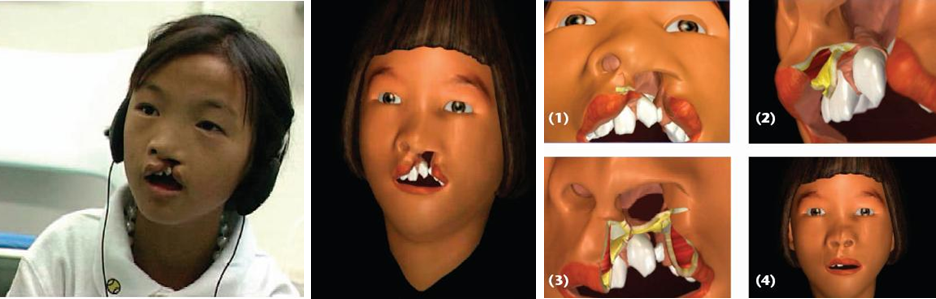
\includegraphics[width=\textwidth]{images/cleft_lip_image}
\caption{Surgical simulation will ideally be used to provide a virtual environment of prototyping procedures as well as for research and development of novel procedures. The images show a subject specific simulated cleft lip and palate repair. Elastic simulation of soft tissues is the primary algorithmic challenge in providing such technologies.}
\label{fig:cleft_lip}
\end{figure}

\section*{Real-time computing}
Real-time simulation refers to the ability to evolve the approximation to an initial boundary value problem in less than a thirtieth of a second. In other words, less than the time it would take to observe the solution on the screen. Traditionally, computation times required for a time step in such problems have been on the order of a few minutes or even a few hours, far short of the thirtieth of a second constraint. However, such performance, should it be allowed, would provide a controllable virtual environment where a user would have the ability to change the forcing and boundary conditions of a simulation in response to real-time observation of the solution. The availability of such functionality for problems in solid and fluid mechanics engenders many new opportunities and applications. For example, imagine an interactive virtual environment where the user interacts with a finite element simulation of biomechanical soft tissues. The governing equations dictate how the tissues respond to external influence from the users. This predictive ability would allow the user to push, pull or even cut/excise portions of the tissue in real time with full confidence that the real life counterpart would behave similarly. This ability could potentially revolutionize the process of training surgical residents and medics by providing a cost effective and scientific alternative to expensive cadaver based training. Imagine the ability to know the outcome of a surgical procedure before it is performed. Reconstructive surgery for severe trauma is unpredictable by the nature of the injuries. The surgeon must design the treatment procedure on a case-by-case basis. With the aid of a predictive simulator the surgeon could perform hypothetical surgical repairs in advance to determine the most likely successful approach. This would significantly reduce complication rates and lead to drastically improved quality of life. See \cite{Sifakis09} for further discussion of the potential benefits of surgical simulation.


\lecture{Introduction to Continuum Mechanics and Elasticity}

\section*{Kinematics}

I will go through the basic continuum mechanics for describing the \emph{initial boundary value problems} (IBVPs) for deformable objects as quickly as possible with an emphasis on only those details necessary for implementing a basic \emph{finite element method} (FEM) type simulation (see the text \cite{Bonet_Wood_2008} for more details). We will quantify the deformation of the objects of interest in terms of the mapping $\bsphi$ between an initial (or material) $\bfB_0 \in \bbR^2$ and current (or deformed) $\bfB_t \in \bbR^2$ configuration (we'll just be covering 2D for simplicity). Let's introduce the convention that points in $\bfB_0$ we label as $\bfX$ and points in $\bfB_t$ we label as $\bfx$ (see Figure~\ref{fig:phi}). I.e. $\bfB_0 = \left\{ \bfX \right\}$ and $\bfB_t = \left\{ \bfx \right\}$ so
\begin{equation*}
\bsphi(\cdot,t) \colon \bfB_0 \to \bfB_t \quad \text{and} \quad \bsphi \left( \bfX, t \right) = \bfx
\end{equation*}
It is also useful to talk about
\begin{equation*}
\bfu(\cdot,t) \colon \bfB_0 \to \bbR^2 \quad \text{where} \quad \bfu \left( \bfX, t \right) = \bsphi \left( \bfX, t \right) - \bfX.
\end{equation*}
We'll refer to this function $\bfu$ as the displacement mapping. We'll also introduce a little more notation here for the derivatives of these mappings. The deformation gradient refers to $\frac{\partial\bsphi}{\partial\bfX}$ and is often denoted with $\bfF$.
\begin{equation*}
\bfF(\cdot,t) \colon \bfB_0 \to \bbR^{2\times2} \quad \text{and} \quad \bfF = \frac{\partial\bsphi}{\partial\bfX}.
\end{equation*}
Index notation for derivatives will be helpful for compactness of expressions. E.g. $F_{ij} = \frac{\partial\phi_i}{\partial X_j} = \phi_{i,j}$ and $\frac{\partial u_i}{\partial X_j} = u_{i,j}$.
\begin{figure}
%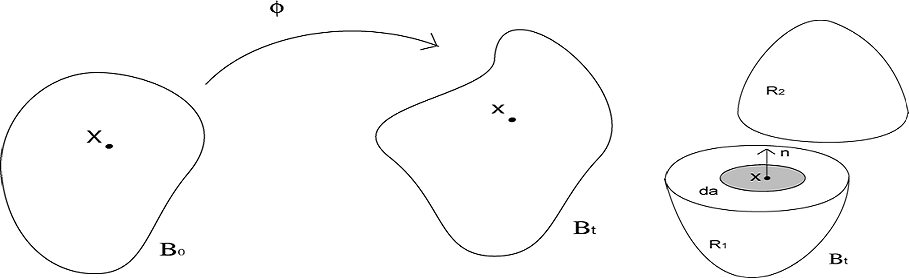
\includegraphics[width=\columnwidth]{images/continuum}
\caption{We will be solving for the mapping between the current configuration and a rest configuration. Stresses will arise via elasticity to resist changes in shape induced by this motion.}
\label{fig:phi}
\end{figure}

\section*{Basic Balance Laws}

Again, I will only present the essential details for getting started with elastodynamics. Our governing equations of motion arise from the basic principles of continuum mechanics, ultimately $F = ma$ applied over our continuum of material $\bfB_0$. This reads as:
\begin{equation*}
\rho_0 \left( \bfX \right) \frac{\partial^2 \bfu}{\partial t^2} = \nabla^{\bfX} \cdot \bfP + \bff^{\text{ext}}.
\end{equation*}
Here, $\rho_0$ is the mass density of the material, $\bff^\text{ext}$ is an externally applied force, and $\bfP$ is the first Piola-Kirchoff Stress which describes the forces of interaction in the material (specifically, $\bfP$ relates the normal of an infinitesimal surface in the material to the forces applied by one side of the material to the other; see Figure~\ref{fig:phi}). We will discuss the form of this stress in the coming sections. For now, note that it is a matrix valued function over the material:
\begin{equation*}
\bfP \colon \bfB_0 \times [0,T] \to \bbR^{2\times2}.
\end{equation*}
For elasticity, we will be relating this quantity to the deformation gradient $\bfF$. It will usually make more sense for us to consider $\bfP$ as a function of $\bfF$, but we will discuss this in the constitutive modeling section. This equation is hyperbolic and roughly like the second order linear wave equation (although the specific nature of $\bfP$ for elasticity will give rise to non-linear equations). It will be useful numerically to consider both the velocities of points of material and the displacements as unknowns. We will use $\bfv \left( \bfX, t \right) = \frac{\partial\bfu}{\partial t} \left( \bfX, t \right)$ to denote the velocity of material point $\bfX$. With this convention, we can rewrite our problem with the equivalent system:
\begin{equation*}
\begin{pmatrix}
\frac{\partial\bfu}{\partial t} \\
\rho_0 \frac{\partial\bfv}{\partial t}
\end{pmatrix}
= \begin{pmatrix}
\bfv \\
\nabla^{\bfX} \cdot \bfP + \bff^{\text{ext}}
\end{pmatrix}.
\end{equation*}

\section*{Elasticity and Constitutive Modeling}

The equations are not yet closed because we still need to determine a relationship between the stress and the state of the material. For elastic materials, this is often referred to as the constitutive or material law. Here, we will focus on hyperelastic materials. The constitutive law for such materials arises from a so-called strain energy density function $\Psi$. Specifically, we define the stress as the derivative of this energy with respect to the deformation gradient $\bfF$:
\begin{equation*}
\Psi \colon \bbR^{2\times2} \to \bbR \quad \text{and} \quad \bfP = \frac{\partial\Psi}{\partial\bfF}.
\end{equation*}
In index notation this is $P_{ij} = \Psi_{,ij}$. In general, the indices following the comma refer to partial differentiation.

The most simplistic model for elasticity is isotropic linear elaticity. In this case, we have
\begin{equation*}
\epsilon_{ij} = \frac{1}{2} \left( F_{ij} + F_{ji} \right) - \delta_{ij} = \frac{1}{2} \left( \frac{\partial u_i}{\partial X_j} + \frac{\partial u_j}{\partial X_i} \right) \quad \text{and} \quad \Psi \left( \bfF \right) = \mu \epsilon_{ij} \epsilon_{ij} + \frac{\lambda}{2} \epsilon_{kk}^2.
\end{equation*}
We are using the convention that repeated indices are summed here and $\delta_{ij}$ is the identity matrix. Differentiating this expression with respect to $\bfF$ gives us the relationship between the stress and the state of the displaced material:
\begin{equation*}
P_{ij} = \Psi_{,ij} = 2 \mu \epsilon_{ij} + \lambda \epsilon_{kk} \delta_{ij} \quad \text{or} \quad \bfP = 2 \mu \bsepsilon + \lambda \operatorname{tr}(\bsepsilon) \bfI.
\end{equation*}
This relationship between the stress and the displacement mapping is enough to close our governing system of equations. I will not give too much motivation for these equations, but note that $\bsepsilon$ is zero when $\bfF$ is skew-symmetric. Also, note that if the displacement is spatially constant, then $\frac{\partial\bfu}{\partial\bfX} = -\bfI$ and hence $\bsepsilon = \bfP = \mathbf{0}$. $\bsepsilon$ is a measure of the strain (or change of shape) in the material. Ideally, we'd like a measure that was invariant under rigid motions $\bsphi$. Unfortunately, the motions just described are only approximately rigid. The approximation is valid if we assume that the deformation is very small. In fact, we can only say that linear elasticity is valid if the deformation is very small. Otherwise, it is not a very good model. That is, it does not accurately describe any elastic materials observed in nature unless the strain is very small. A more general expression of a rigid body motion is that the deformation gradient is orthogonal. I.e., that $\bfF^T \bfF = \bfI$. In fact, more appropriate strain measures for large deformation elasticity are the right and left Cauchy-Green strain tensors: $\bfG_R = \bfF^T \bfF - \bfI$ and  $\bfG_L = \bfF \bfF^T - \bfI$, respectfully. Note that this measure is quadratic in the deformation. This will lead to nonlinear governing equations and complicate considerably the process of running our simulation. In other words, if we want to simulate large tissues that undergo significant deformation (as we would need in virtual surgery), we'll be stuck with nonlinear governing equations.

Arguably, the most simplistic model for large deformation elasticity is the \emph{Neo-Hookean} model. The hyperelastic strain energy density for such materials is given by the following equation
\begin{subequations}
\begin{equation*}
\Psi \left( \bfF \right) = \frac{\mu}{2} \left( F_{ij} F_{ji} - 2 \right) - \mu \log(J) + \frac{\lambda}{2} \log(J)^2
\end{equation*}
\begin{equation*}
\bfP \left( \bfF \right) = \mu \bfF + \left( \lambda \log(J) - \mu \right) \bfF^{-T}
\end{equation*}
\end{subequations}
where  $J$ is the determinant of the deformation gradient
\begin{equation*}
J = \det \left( \bfF \right).
\end{equation*}
The log term in this equation is there to resist changes in volume. The $\lambda$ and $\mu$ terms can be set as in linear elasticity. The most intuitive way to set these parameters is from the Young's modulus $K$ and Poisson's ratio $\nu$. This relationship is
\begin{equation*}
\lambda = \frac{K \nu}{(1 + \nu)(1 - 2\nu)} \quad \text{and} \quad \mu = \frac{K}{2 (1 + \nu)}.
\end{equation*}
The Young's modulus is a measure of the stiffness of the material and should be larger than zero (typically around $1000$ for our exercises). The Poisson's ratio is a measure of the incompressibility of the material and should be between 0 and $\frac{1}{2}$ (with $\nu = \frac{1}{2}$ being the limit of an incompressible material; note that $\lambda$ goes to $\infty$ in this case).

\begin{figure}
%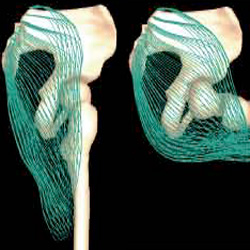
\includegraphics[width=.5\columnwidth]{images/muscle_biomechanics_2005}
\caption{Constitutive models for muscle, tendon, ligament and many other tissues must be anisotropic to accurately reflect the natural fibrous structure of these materials. In such cases, we must represent a fiber field defined over the material configuration of the material as shown above in a rectis femoris muscle.}
\label{fig:fibers}
\end{figure}

The models described so far are both isotropic. That is, the elastic response to deformation is the same regardless of which direction the material is stretched in. This is not very accurate for many fibrous tissues in the anatomy. In these cases, we need an auxiliary function $\bfg \colon \bfB_0 \to \bbR^2$ that describes the local fiber direction in the material configuration of the tissue (see Figure~\ref{fig:fibers}). The specialized response in the fiber direction can be incorporated by changing the original isotropic strain energy density to include a term based on the stretching in the fiber direction: $\bfg^T \bfF^T \bfF \bfg$. That is, the modification looks like
\begin{equation*}
\Psi \left( \bfF \right) = \Psi_{\text{iso}} \left( \bfF \right) + \Psi_{\text{fiber}} \left( \bfg^T \bfF^T \bfF \bfg \right).
\end{equation*}

\begin{figure}
%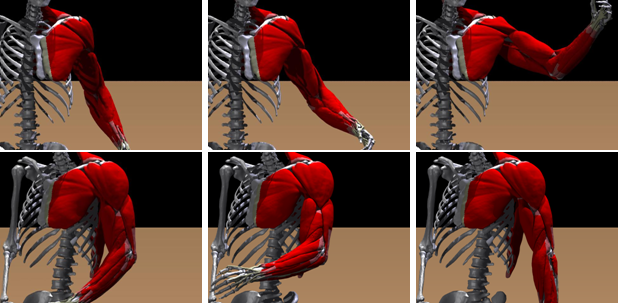
\includegraphics[width=\columnwidth]{images/muscles}
\caption{Simulation of elasticity for the musculoskeletal system.}
%\label{fig:mucles}
\end{figure}

\section*{Equilibrium and Weak Form}

We can get an idea for how to treat the spatial discretization of the partial differential equation by first considering elastic equilibrium (or quasistatic) problems where the inertial terms in the governing equations are negligible (see \cite{Teran05a} for more details). In this case we can solve directly for the displacement (i.e., we don't need to store the velocities as well). Ignoring inertia, our governing equations are then
\begin{equation*}
-\nabla^{\bfX} \cdot \bfP = \bff^{\text{ext}} \quad \text{or} \quad -P_{ij,j} = f^{\text{ext}}_i.
\end{equation*}
This can be read as the row wise divergences of the matrix $\bfP$ balance the different components of the applied forces. We'll mainly be considering \emph{finite element method} (FEM) type discretizations in these notes, so we'll look at the weak form here to get started with that. Taking a class of test functions $\bfw \colon \bfB_0 \to \bbR^2$, we take the dot product with both sides of the governing equations and integrate over $\bfB_0$ to get
\begin{subequations}
\begin{equation*}
-\int_{\bfB_0} w_i P_{ij,j} d\bfX = \int_{\bfB_0} w_i f^{\text{ext}}_i d\bfX
\end{equation*}
\begin{equation*}
-\int_{\bfB_0} \left( w_i P_{ij} \right)_{,j} - w_{i,j} P_{ij} d\bfX = \int_{\bfB_0} w_i f^{\text{ext}}_i d\bfX
\end{equation*}
\begin{equation*}
\int_{\bfB_0} w_{i,j} P_{ij} d\bfX = \int_{\partial\bfB_0} w_i P_{ij} n_j d\bfS \left( \bfX \right) + \int_{\bfB_0} w_i f^{\text{ext}}_i d\bfX.
\end{equation*}
\end{subequations}
We'd then just assume that the bottom equations hold for all suitable $\bfw$ for the weak form. Furthermore, the quantity $P_{ij} n_j$ would be supplied as a boundary condition (this would be the external loading on the material). A FEM discretization would then be done by setting up a space of interpolating functions over a mesh and considering the weak form over this finite dimensional space.

\section*{1D Elasticity}

To provide an introductory example, I will cover the case of 1D elasticity (I will assume some basic knowledge of FEM). Here, we'll first assume the material is linearly elastic. In that case,
\begin{equation*}
P(X) = \left( 2 \mu - \lambda \right) \frac{\partial u}{\partial X}
\end{equation*}
and the equilibrium equation is just Poisson's equation:
\begin{equation*}
-\left( 2 \mu - \lambda \right) \frac{\partial^2 u}{\partial X^2} = f^{\text{ext}}.
\end{equation*}
Thus, we can just use a continuous piecewise linear interpolation space of a uniform discretization of our material (which I will assume for simplicity is just some interval $(a,b)$). In this case, we will ultimately just be solving a Poisson equation for the unknown deformation field. This is only the case in 1D. If we assume that each node in the discrete domain has an associated interpolating function $N_i$, then the FEM discretized linear system is
\begin{subequations}
\begin{equation*}
A_{ij} u_j = F^{\text{ext}}_i + g_i \quad \text{where} \quad A_{ij} = \left( 2 \mu - \lambda \right) \int_a^b \frac{\partial N_i}{\partial X}\frac{\partial N_j}{\partial X} dX,
\end{equation*}
\begin{equation*}
F^{\text{ext}}_i = \int_a^b f^{\text{ext}} N_i dX, \quad g_i = N_i(b) P(b) - N_i(a) P(a)
\end{equation*}
\end{subequations}
(where we assume that $P(a)$ and $P(b)$ were already given). Now, let's consider the case of Neo-Hookean elasticity. In this case, our discretization of the weak form will give rise to a nonlinear system of equations for our displacements $u_i$:
\begin{equation*}
q_i \left( \vec{u} \right) = \int_a^b \frac{\partial N_i}{\partial X} P(F(u(X))) dX - F^{\text{ext}}_i + g_i = 0
\end{equation*}
where $u(X) = u_i N_i(X)$ (again, where repeated indices imply sumation). For Neo-Hookean materials in 1D, we have
\begin{equation*}
P(F(u(X))) = \mu \left( \frac{\partial u}{\partial X} + 1 \right) + \left( \lambda \text{log} \left( \frac{\partial u}{\partial X} + 1 \right) - \mu \right) \frac{1}{\frac{\partial u}{\partial X} + 1}.
\end{equation*}
We can think of $\vec{q} : \bbR^n \to \bbR^n$ as a nonlinear function that we need to find a zero of. We'll use Newton's method to iteratively improve our approximate solution (here, I am assuming $\vec{u}^k \in \bbR^n$ is our current approximation to the vector of discrete displacements) as:
\begin{subequations}
\begin{equation*}
\frac{\partial q_i}{\partial u_j} \left( \vec{u}^k \right) \Delta{u}_j + q_i \left( \vec{u}^k \right) = 0,
\end{equation*}
\begin{equation*}
u_i^{k+1} \leftarrow u_i^{k} + \Delta{u}_i.
\end{equation*}
\end{subequations}
The linearization of the discrete equilibrium equations can be a little tricky, so it will be good to first consider it in 1D. The general idea is to linearize the stress with respect to the deformation gradient, then linearize the deformation gradient with respect to discrete degrees of freedom.
\begin{equation*}
\frac{\partial q_i}{\partial u_j} \left( \vec{u} \right) = \int_a^b \frac{\partial N_i}{\partial X} \frac{\partial P}{\partial F} \left( F \left( \vec{u} \right) \right) \frac{\partial F}{\partial u_j} dX = \int_a^b \frac{\partial N_i}{\partial X} \frac{\partial P}{\partial F} \left( F \left( \vec{u} \right) \right) \frac{\partial N_j}{\partial X} dX
\end{equation*}
since $u(X) = u_i N_i(X)$ and $F(X) = \frac{\partial u}{\partial X}(X) + 1 = u_i \frac{\partial N_i}{\partial X}(X) + 1$. Note that the linearized system is just a spatially varying Poisson equation. However, it should be noted that for such equations we must typically require the coefficients remain positive throughout the domain. This will not always happen and can lead to difficulties with robustness. We will discuss this issue in the next section.

\begin{figure}
%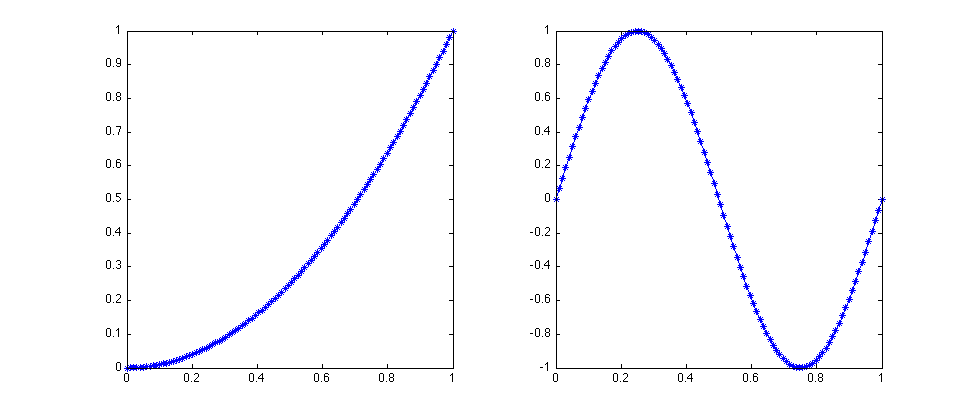
\includegraphics[width=\columnwidth]{images/elasticity_1d}
\caption{The image at the left shows an acceptable solution for the deformation $\phi$ (namely, $\phi(X) = X^2$). The solution at the right shows one that would produce inverted material (namely, $\phi(X) = \sin \left( 2 \pi X \right)$).}
\label{fig:inversion}
\end{figure}

\section*{Inversion}

The deformation mapping $\bsphi$ must be a bijection (one-to-one and onto) if we are to strictly apply the principles of continuum mechanics. This precludes many solutions you might otherwise expect to see. For example, for the 1D case, the solution must never have a derivative less than or equal to zero. I.e. many functions we are used to solving for (see Figure~\ref{fig:inversion}) are not, strictly speaking, allowable. Unfortunately, this constraint will not always be naturally achieved by our discretization. For some models (e.g. linear elasticity) it is okay that the discrete solution does not satisfy the inversion constraint. For others like Neo-Hookean, we would end up taking the natural log of a negative number. This log term is there to prevent excessive compression. However, it has the consequence that our equations become incredibly stiff under compression. Such behavior can be very problematic numerically and must be avoided in a surgical simulator. A general approach to improving robustness to discretely inverted (i.e., non-bijective) deformation mappings was developed in \cite{Irving06}. I will not go through all of the details for the sake of time. However, I will show how we can apply the principles developed in this work to our simple Neo-Hookean model.

\begin{figure}
%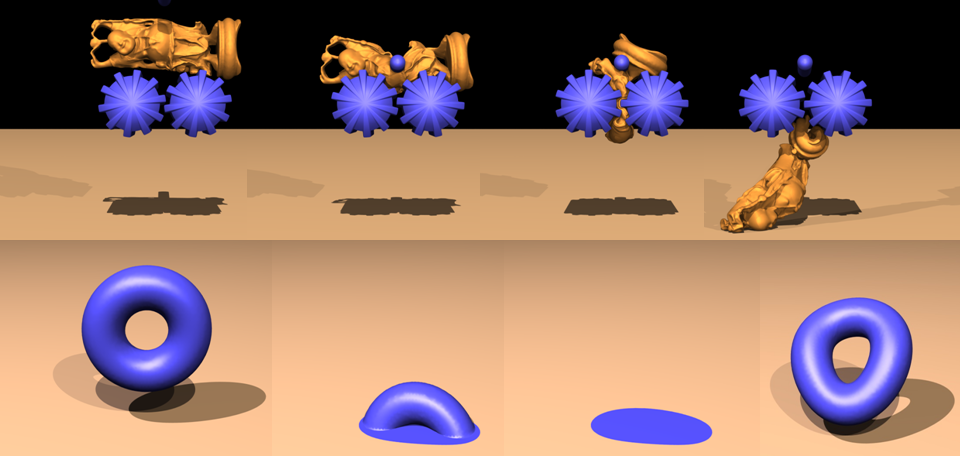
\includegraphics[width=\columnwidth]{images/buddha_gears}
\caption{These images show the the algorithm of \cite{Irving06} in action. This algorithm is based on removing the bijection constraint from continuum mechanics in the discrete setting to provide robustness to large deformation.}
%\label{fig:inversion2}
\end{figure}

The problematic term in the Neo-Hookean model is the natural log. If we replace the log with another function $r$, we can improve the robustness of our numerical simulation to inversion. This function should look very nearly like the natural log around $J = 1$ to prevent loss of accuracy, but should not have a singularity at $J = 0$. We can do this by taking $r$ to be the cubic Taylor expansion of the log around $J = 1$ (see Figure~\ref{fig:inversion3}). With this choice, we have the following expressions for the Neo-Hookean hyperelastic strain energy density and first Piola-Kirchoff stresses:
\begin{subequations}
\begin{equation*}
\Psi \left( \bfF \right) = \frac{\mu}{2} \left( F_{ij} F_{ji} - 2 \right) - \mu r(J) + \frac{\lambda}{2} r(J)^2
\end{equation*}
\begin{equation*}
\bfP \left( \bfF \right) = \mu \bfF + \left( \lambda r(J) -\mu \right) r'(J) \begin{pmatrix} F_{22} & -F_{12} \\
-F_{21} & F_{11} \end{pmatrix}.
\end{equation*}
\end{subequations}
In Figure~\ref{fig:inversion3}, we see the effect of this modification in 1D. This new model is well-defined through inversion, but accurately reflects the original model when very near the undeformed configuration. We can make further adjustments to prevent problematic values of $\frac{\partial P}{\partial F}$ (e.g. we wanted this to be positive for our 1D example). The treatment of these terms is addressed in \cite{Teran05a}.

\begin{figure}
%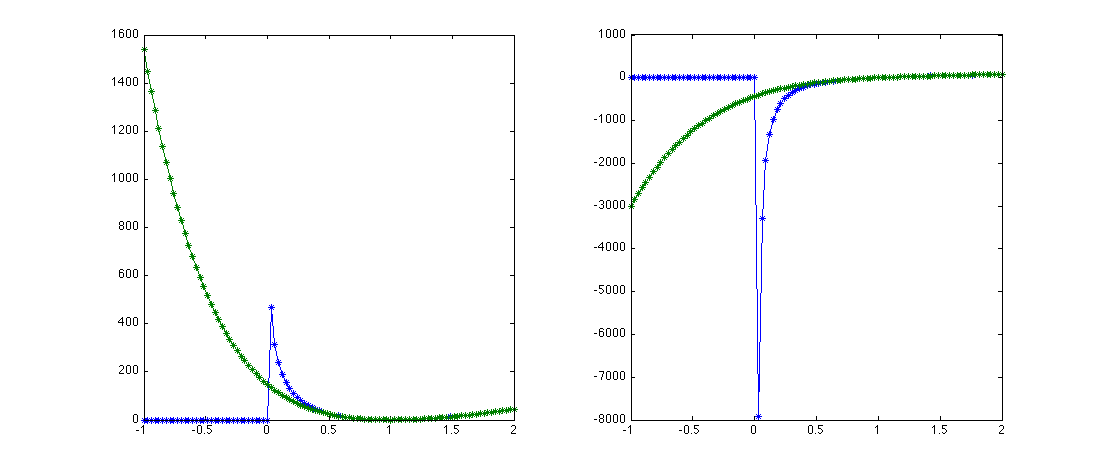
\includegraphics[width=\columnwidth]{images/invertible_neo_hookean}
\caption{The plots at the left are of the hyperelastic energy density of the 1D Neo-Hookean model. The plots at the right are of the 1D Neo-Hookean stresses. The blue curves are the unmodified Neo-Hookean model, the green curves result from replacing the log with it's cubic Taylor expansion around $J = 1$. These are preferable for the sake of robustness.}
\label{fig:inversion3}
\end{figure}

\section*{Time Stepping}

In general, our simulator will run the following loop:
\begin{equation}
\begin{array}{lc}
\text{for} \ n = 0 : N_\text{final} \\
\quad \bullet \ \text{get user boundary condition input} \\
\quad \bullet \ t \leftarrow t + \Delta{t} \\
\quad \bullet \ \text{solve nonlinear system for displacements and velocities} \\
\quad \bullet \ \text{render solution to screen}\\
\text{end}
\end{array}
\end{equation}
The key factor is that the nonlinear system must be solved in less than one thirtieth of a second to maintain an interactive simulation rate. An example of a discretization of this system that allows for inertia is the following. Let $\vec{u}^m \in \bbR^n$ represent the spatially discrete displacements at time $m$ and let $\vec{v}^m \in \bbR^n$ represent the spatially discrete velocities. We can implement backward Euler by saying
\begin{equation*}
\vec{v}^{m+1} = \frac{1}{\Delta t} \left( \vec{u}^{m+1} - \vec{u}^m \right)
\end{equation*}
and
\begin{equation*}
\rho_0 \frac{1}{\Delta t} \left( \frac{1}{\Delta t} \left( \vec{u}^{m+1} - \vec{u}^m \right) - \vec{v}^m \right) = \nabla^{\bfX} \cdot \bfP \left( \bfF \left( \vec{u}^{m+1} \right) \right) + \bff^{\text{ext}}
\end{equation*}
where we solve this final system by following a similar FEM procedure to the quasistatic case for $\vec{u}^{m+1}$. Specifically, we'd get
\begin{align*}
q^a_i \left( \vec{u}^{m+1} \right)
& = M_{ai;bj} u^{m+1}_{bj} \\
& \quad {} + \Delta t^2 \int_{\bfB_0} N^a_{,j} P_{ij} d\bfX \\
& \quad {} - M_{ai;bj} \left( u^{m+1}_{bj} + \Delta{t} v^m_{bj} \right) \\
& \quad {} - \int_{\partial\bfB_0} N^a P_{ij} n_j d\bfS \left( \bfX \right) \\
& \quad {} - \int_{\bfB_0} N^a f^{\text{ext}}_i d\bfX
\end{align*}
and $M_{ai;bj}=\int_{\bfB_0} N^a \rho_0 N^b \delta_{ij} d\bfX$.

\lecture{Numerical Solutions of the Equations of Elasticity}

This lecture provides details and exercises pertaining to the implementation of numerical solvers for the equations of elasticity. We begin with a review of the Finite Element Method (FEM) as it applies to Poisson's equation. We will then apply this framework to numerically solve the equations of elasicity, first in dimension $d = 1$ with quasistatic evolution, then in dimension $d = 2$ with inertial effects included.

\section{Numerical Solution of Poisson's Equation via the Finite Element Method}

Let us consider numerical solutions of (variable coefficient) Poisson's equation:
\begin{subequations}
\begin{align}\label{eq:poisson.strong}
-\nabla \cdot \left( \beta \nabla u \right) & = f \quad \in \Omega \\
u & = p \quad \in \partial \Omega_d \\
\beta \nabla u \cdot \hat{n} & = q \quad \in \partial \Omega_n
\end{align}
\end{subequations}
Here, $\Omega \subset \bbR^d$ is open; $\partial \Omega_d$ and $\partial \Omega_n$ partition the boundary of $\Omega$ and define where \emph{Dirichlet} ($d$) and \emph{Neumann} ($n$) boundary conditions are applied, respectively; $\hat{n}$ is the outward-pointing unit normal on $\partial \Omega_n$; $\beta, f \colon \Omega \to \bbR$, $p \colon \partial \Omega_d \to \bbR$, and $q \colon \partial \Omega_q \to \bbR$ are given, and $\beta$ is bounded below by some positive number; and the goal is to solve for the unknown function $u \colon \Omega \to \bbR$. For now, we'll ignore the details of the function spaces that $u$, $\beta$, $f$, $p$, and $q$ are assumed to belong in.

For the numerical solution of \eqref{eq:poisson.strong}, we'll use a discretization based on the Finite Element Method (FEM). Briefly, an FEM discretization focuses on the weak formulation of the partial differential equation. The derivation involves multiplying the differential equation by a test function (chosen from some suitable function space), integrating by parts, and applying boundary conditions:
\begin{subequations}
\begin{align}
& -\nabla \cdot \left( \beta \nabla u \right) = f \\
\Rightarrow & \int_{\Omega} -\nabla \cdot \left( \beta \nabla u \right) v = \int_{\Omega} f v \\
\Rightarrow & \int_{\Omega} \beta \nabla u \cdot \nabla v =
    \int_{\Omega} f v + \int_{\partial \Omega} \left( \beta \nabla u \cdot \hat{n} \right) v \label{eq:poisson.weak.c} \\
\Rightarrow & \int_{\Omega} \beta \nabla u \cdot \nabla v = \int_{\Omega} f v + \int_{\partial \Omega_n} q v \label{eq:poisson.weak.d}
\end{align}
\end{subequations}
where the derivation from \eqref{eq:poisson.weak.c} to \eqref{eq:poisson.weak.d} is possible by stipulating that $v \equiv 0$ on $\partial \Omega_d$. Clearly, then, if $u$ satisfies \eqref{eq:poisson.strong}, then $u$ also satisfies \eqref{eq:poisson.weak.d} for all appropriate $v$. Under suitable conditions, it turns out to be the case that the converse holds as well. Since \eqref{eq:poisson.weak.d} involves only first order derivatives in $u$, its analysis is often preferable to \eqref{eq:poisson.strong}.

We then suppose that $u$ can be approximated by a function in a finite-di\-men\-sion\-al function space (the \emph{(discretized) solution space}) (e.g., continuous piecewise linear functions over some tessellation of $\Omega$), i.e., $u \approx \tilde{u} = \sum_j u_j e_j$ for basis elements $\left\{ e_j \right\}$. Likewise, $v$ is selected from some other (often related) finite-dimensional function space (the \emph{(discretized) test space}), thus giving a system of equations for the coefficients $u_j$. For example, if $v$ is taken from the same space as $\tilde{u}$, and we let $v$ be, in turn, each of the basis functions, then we obtain
\begin{equation}\label{eq:poisson.system.i}
\sum_j \left( \int_{\Omega} \beta \nabla e_j \cdot \nabla e_i \right) u_j = \int_{\Omega} f e_i + \int_{\partial \Omega_n} q e_i
\end{equation}
for all $i$, which may be expressed as a linear system of equations:
\begin{equation}\label{eq:poisson.system.a}
A \vec{u} = \vec{b},
\end{equation}
where
\begin{subequations}\label{eq:poisson.system.b}
\begin{align}
A_{ij} & = \int_{\Omega} \beta \nabla e_i \cdot \nabla e_j \label{eq:poisson.system.Aij} \\
\vec{u}_i & = u_i \\
\vec{b}_i & = \int_{\Omega} f e_i + \int_{\partial \Omega_n} q e_i \label{eq:poisson.system.bi}
\end{align}
\end{subequations}
Strictly speaking, the above is only correct if $v$ varies \emph{precisely} throughout the same function space which $\tilde{u}$ belongs to. This is generally not the case. For example, in the presence of Dirichlet boundary conditions, $\tilde{u}$ will generally be nonzero along $\Omega_d$, however $v$ will be chosen from a function space which vanishes along $\Omega_d$ (hence these functions spaces will only align under homogeneous Dirichlet boundary conditions). How this manifests itself in the linear system will be investigated in the exercises.

Note that the sparsity of $A$ is directly related to the overlap of the supports of the $e_j$'s. Typically we choose the $e_j$'s such that the support of one basis element overlaps the supports of only a small constant number of other basis elements, in which case $A$ will have a number of nonzero entries proportional to the number of basis elements.

Let's now focus on dimension $d = 1$ and use \emph{linear finite elements}. Let $\Omega$ be an interval $(a,b)$, and let $\{x_j\}$ be grid points in $(a,b)$, with $a = x_0 < x_1 < \dotsm < x_n = b$. Often times, the $x_j$'s will be equally spaced, which makes the analysis simpler, but it's not necessary. We'll take $\tilde{u}$ (the discretized solution) and $v$ (the discretized test function) to be continuous and \emph{piecewise linear} on each segment $\left( x_{j-1}, x_j \right)$, with $v(a)$ and/or $v(b)$ vanishing if a Dirichlet condition is specified at $a$ and/or $b$, respectively. This space of continuous piecewise linear functions is spanned by the \emph{nodal basis functions} (also called ``hat'' functions, because of the shape of their graphs) $e_j$, (uniquely) defined such that
\begin{equation}\label{eq:poisson.1d.ej}
e_j(x_k) = \delta_{jk} = \begin{cases} 1, & j = k \\ 0, & j \neq k \end{cases}
\end{equation}

\subsection{Exercises}

Unless otherwise noted, assume dimension $d = 1$ linear finite elements with the basis $\{e_j\}$ given by \eqref{eq:poisson.1d.ej}, although these results extend to higher order and higher dimensional finite elements.

\begin{enumerate}

\item Here is one way to incorporate the Dirichlet boundary conditions into \eqref{eq:poisson.system.b}. For concreteness, suppose $\Omega_d = \{a\}$ (with $\Omega = (a,b)$). Then we still have $\tilde{u} = \sum_{j = 0}^n u_j e_j$, but our space of test functions $\{v\}$ is slightly smaller, $\operatorname{span} \{ e_1, \dotsc, e_n \}$, to ensure that $v(a) = 0$. Thus we obtain $n$ equations of the form \eqref{eq:poisson.system.i}, plus one more equation from the Dirichlet boundary condition ($u_0 = u(a)$). This (ostensibly) gives enough equations to solve for the $n + 1$ coefficients $\{u_j\}$.

Another conceptual way to incorporate the Dirichlet boundary conditions is to consider the function $w = u - u(a) e_0$, which satisfies a similar Poisson problem as $u$ but now with homogeneous Dirichlet boundary conditions. Thus, the space of test functions $\{v\}$ and the solution space of $w$ coincide, and one may use eqs \eqref{eq:poisson.system.b} directly.

In practice, one can actually just ignore the Dirichlet boundary conditions when initially computing the entries of $A$ and $\vec{b}$ (i.e., just use \eqref{eq:poisson.system.Aij} and \eqref{eq:poisson.system.bi}), then ``correct'' $A$ and $\vec{b}$ to account for the Dirichlet boundary conditions afterwards. Describe a \emph{simple} algorithm to effect this ``correction'' procedure. Try to keep $A$ symmetric.

\item Show that the linear system \eqref{eq:poisson.system.a} has a unique solution if one specifies Dirichlet boundary conditions at either $x = a$ or $x = b$ or both (i.e., $u(a) = u_a$ and/or $u(b) = u_b$). For simplicity, you may assumed $\beta \equiv 1$. What happens if both boundary conditions are Neumann? Specifically address the conditions which $\vec{b}$ must satisfy, how this translates into a condition on $f$, and ``how uniquely'' $\tilde{u}$ is determined.

\item Compute the integral in \eqref{eq:poisson.system.Aij} when $\beta \equiv 1$. If you wish, for simplicitly, you may assume the $x_j$'s are equally spaced, i.e., $x_j = a + j h$, where $h = (b - a)/n$. What is the structure of the matrix $A$ (e.g., describe the sparsity)?

\item Give an expression to reasonably approximate the integrals in \eqref{eq:poisson.system.Aij} and \eqref{eq:poisson.system.bi} for aribtrary $\beta$, $f$, and $q$ (assume $\beta$ and $f$ are sufficiently ``well-behaved''). You may have to consider boundary and interior grid vertices separately.

\item Write some code (e.g., a Matlab script) to solve the following boundary value problem using linear finite elements:
\begin{align*}
-\left( \left( 1 + x \right) u'(x) \right)' & = \left( 1 + x \right)^{-2} \quad x \in (0, 1) \\
u(0) & = 1 \\
\left( 1 + (1) \right) u'(1) & = -1/2
\end{align*}

\item The FEM terminology for the matrix $A$ in \eqref{eq:poisson.system.a} is the \emph{(global) stiffness matrix} (the meaning of the term ``global'' will become obvious shortly). With dimension $d = 1$ linear finite elements, it is relatively straightforward to compute the entries of the stiffness matrix, even given that one has to account for differences between boundary and interior grid vertices. However, the situation becomes more complicated with higher order or higher dimensional finite elements, and it becomes tedious to consider all the special boundary cases. As such, it is common practice to assemble the global stiffness matrix element by element (i.e., cell by cell), with each element contributing partially to several entries of the global stiffness matrix. The collection of these contributions from a single element may be put into a small matrix, the \emph{local stiffness matrix} for that element. The computation of the local stiffness matrix is identical to that of the global stiffness matrix upon replacing the integrations over $\Omega$ with integrations localized over the element. For example, back to dimension $d = 1$ linear finite elements, the local stiffness matrix over $I_j = \left( x_{j-1}, x_j \right)$ would consist of $2^2$ (nonzero) entries (since only $2$ basis functions are supported on $I_j$). Each of these entries would be added to accumulated global stiffness matrix entries:
\begin{align*}
A_{j-1,j-1}          & {} +\!\!= \int_{I_j} \beta \nabla e_{j-1} \cdot \nabla e_{j-1} \\
A_{j-1,j}, A_{j,j-1} & {} +\!\!= \int_{I_j} \beta \nabla e_{j-1} \cdot \nabla e_j \\
A_{jj}               & {} +\!\!= \int_{I_j} \beta \nabla e_j \cdot \nabla e_j
\end{align*}
This suggests the following procedure to build the (global) stiffness matrix $A$. First, initialize the sparsity pattern of $A$ (with zeros). Then iterate through each element and add the contributions of the element's local stiffness matrix to the corresponding entries in $A$.

Verify this procedure computes the same stiffness matrix as before, and modify your program from Exercise 5 to build the stiffness matrix in this fashion.

\end{enumerate}

\section{Neo-Hookean Elasticity with Quasistatics Evolution in Dimension~1}

Let us now consider the numerical solution of the equations of elasticity with the Neo-Hookean constitutive model. To begin, for simplicity, we will consider using quasistatic evolution in dimension $d = 1$. The subsequent section will extend this into dimension $d = 2$ and add inertial effects.

\subsection{Elasticity}

Recall that the equations of elasticity are given by the boundary value problem
\begin{subequations}\label{eq:elasticity.i}
\begin{align}
\rho_0 \left( \bfX \right) \frac{\partial^2 \bfu}{\partial t^2} & = \nabla^{\bfX} \cdot \bfP + \bff^{\text{ext}} \quad \in \Omega(t) \\
\bfu(t,\cdot) & = \bfg(t,\cdot) \quad \in \partial \Omega_d(t) \\
\left( \bfP \cdot \mathbf{\hat{n}} \right) (t,\cdot) & = \bfh(t,\cdot) \quad \in \partial \Omega_n(t)
\end{align}
\end{subequations}
where $\rho_0 \colon \Omega_0 \to \bbR$ is the mass density (as a function of $\bfX$, the undeformed coordinates); $\bfu \colon \Omega_0 \to \Omega(t), \bfX \mapsto \bsphi \left( \bfX \right) - \bfX$ is the unknown displacement; $\bfP$ is the first Piola-Kirchoff stress (which takes a specific form for Neo-Hookean, to be given later); $\bff^{\text{ext}}$ is the given (external) force; and $\bfg$ and $\bfh$ specify the Dirichlet and Neumann boundary conditions, respectively. For simplicity, we'll assume a uniform mass density, i.e., $\rho_0 \equiv 1$.

\subsection{Neo-Hookean Constitutive Model}

The Neo-Hookean constitutive model relates the stress $\bfP$ to the deformation gradient $\bfF := \frac{\partial\bsphi}{\partial\bfX}$ via
\begin{subequations}
\begin{align}
\Psi \left( \bfF \right) & := \frac{\mu}{2} \left( F_{ij} F_{ji} - 2 \right) - \mu \log J + \frac{\lambda}{2} \log^2 J, \label{eq:neo-hookean.strain.energy} \\
\bfP \left( \bfF \right) := \frac{\partial \Psi}{\partial \bfF} & = \mu \bfF + \left( \lambda \log J - \mu \right) \bfF^{-T}.
\end{align}
\end{subequations}
(Recall that $J := \det \bfF$.) This manifests itself in dimension $d = 1$ in terms of the displacement $u$ as
\begin{equation*}
P(u) = \mu \left( \frac{du}{dX} + 1 \right) + \left( \lambda \log \left( \frac{du}{dX} + 1 \right) - \mu \right) \frac{1}{\frac{du}{dX} + 1}.
\end{equation*}

\subsection{Inversion-Robust Neo-Hookean}

Neo-Hookean as formulated above will not be robust to element inversions, due to the $\log J$ terms. To remedy this, we replace the logarithm in \eqref{eq:neo-hookean.strain.energy} with a cubic Taylor approximation around $1$:
\begin{subequations}\label{eq:r}
\begin{align}
\begin{split}
r(x) & = (x - 1) - \frac{1}{2} (x - 1)^2 + \frac{1}{3} (x - 1)^3 \\
     & = -\frac{11}{6} + 3 x - \frac{3}{2} x^2 + \frac{1}{3} x^3,
\end{split} \\
\begin{split}
r'(x) & = 1 - (x - 1) + (x - 1)^2 \\
      & = 3 - 3 x + x^2.
\end{split} \\
\begin{split}
r''(x) & = -1 + 2 (x - 1) \\
       & = -3 + 2 x.
\end{split}
\end{align}
\end{subequations}
This gives
\begin{align*}
\Psi \left( \bfF \right) & = \frac{\mu}{2} \left( F_{ij} F_{ji} - 2 \right) - \mu r(J) + \frac{\lambda}{2} r(J)^2, \\ \bfP \left( \bfF \right) = \frac{\partial \Psi}{\partial \bfF} & = \mu \bfF + \left( \lambda r(J) - \mu \right) r'(J) \frac{\partial J}{\partial \bfF}.
\end{align*}
Again, specializing this for $d = 1$ dimension, we obtain
\begin{equation}\label{eq:P.1d}
P(u) = \mu \left( \frac{du}{dX} + 1 \right) + \left( \lambda r \left( \frac{du}{dX} + 1 \right) - \mu \right) r' \left( \frac{du}{dX} + 1 \right).
\end{equation}

\subsection{Quasistatic Evolution}

We begin by studying \eqref{eq:elasticity.i} at equilibrium, which is the basis for quasistatic evolution. This reduces the equations to
\begin{equation}\label{eq:elasticity.quasistatic}
-\nabla^{\bfX} \cdot \bfP = \bff^{\text{ext}}.
\end{equation}
The equivalent weak formulation is
\begin{equation*}
\int_{\Omega_0} w_{i,j} P_{ij} d\bfX = \int_{\partial \Omega_n} w_i h_i dS \left( \bfX \right) + \int_{\Omega_0} w_i f_i^{\text{ext}} d\bfX
\end{equation*}
for all test functions $\bfw$. Recall that summation over repeated indices is implied, and comma'ed indices indicate differentiation.

As for Poisson, we let the coordinates of $\bfw$ vary over the nodal basis functions $N_i$. In dimension $d = 1$, this reduces to the system of equations
\begin{subequations}\label{eq:elasticity.quasistatic.weak.1d}
\begin{align}
0 = q_i \left( \vec{u} \right) & := \int_a^b \frac{\partial N_i}{\partial X} P(F(u(X))) dX - b_i; \label{eq:elasticity.quasistatic.weak.1d.qi} \\
b_i & := \int_a^b N_i f^{\text{ext}} dX + \text{[Neumann boundary terms]} \label{eq:elasticity.quasistatic.weak.1d.bi}
\end{align}
\end{subequations}
for each grid vertex $i$, where $u := u_i N_i$. The Neumann boundary terms consist of neither, one, or both of $N_i(b) h(b)$ and/or $-N_i(a) h(a)$, depending on whether $b$ and/or $a$, respectively, belong to $\partial\Omega_n$.

For Neo-Hookean, $P$ depends \emph{non-linearly} on the displacement $u$, hence one must use a non-linear solver, such as Newton iteration, to solve \eqref{eq:elasticity.quasistatic.weak.1d} for $\vec{u} := \left( u_i \right)$. The Newton step looks like
\begin{subequations}
\begin{equation*}
\frac{\partial q_i}{\partial\vec{u}} \left( \vec{u} \right) \Delta \vec{u} + q_i \left( \vec{u} \right) = 0;
\end{equation*}
\begin{equation*}
\vec{u} \leftarrow \vec{u} + \Delta \vec{u}
\end{equation*}
\end{subequations}
where
\begin{equation*}
\frac{\partial q_i}{\partial u_j} \left( \vec{u} \right) = \int_a^b \frac{\partial N_i}{\partial X} \frac{\partial P}{\partial F} \left( F(u) \right) \frac{\partial N_j}{\partial X} dX
\end{equation*}
Thus, the computation of $\Delta \vec{u}$ in each Newton iteration amounts to solving a variable coefficient Poisson problem. The coefficient is $\partial P/\partial F$, which we can express via \eqref{eq:P.1d} as
\begin{equation*}
\frac{\partial P}{\partial F} = \mu + \lambda r' \left( \frac{du}{dX} + 1 \right)^2 + \left( \lambda r \left( \frac{du}{dX} + 1 \right) - \mu \right) r'' \left( \frac{du}{dX} + 1 \right).
\end{equation*}
This gives all the necessary pieces to implement a quasistatic evolution of the equations of elasticity \eqref{eq:elasticity.i}.

\subsection{Implementation}

Let us assume a regular grid on $(a,b)$, such that we have $n$ grid vertices $x_i := a + (i - 1) \Delta x$, $\Delta x := (b - a)/(n - 1)$, and $i$ ranges from $1$ to $n$, inclusive. We break the implementation of such a solve into several steps, outlined below and expounded upon in the subsequence subsubsections.
\begin{itemize}
\item Compute $\vec{b} := \left( b_1, \dotsc, b_n \right)$ (from \eqref{eq:elasticity.quasistatic.weak.1d.bi}).
\item Implement a procedure to compute $\vec{q} := \left( q_1, \dotsc, q_n \right)$ (from \eqref{eq:elasticity.quasistatic.weak.1d.qi}).
\item Implement a procedure to compute $\partial q/\partial\vec{u}$.
\item Solve for the Newton increment $\Delta \vec{u}$.
\end{itemize}
We provide psuedocode for all steps in a syntax similar to Matlab or Octave.

\subsubsection{Compute $\vec{b}$}

We begin by considering the computation of $\vec{b}$. This is a natural place to start because, first, it remains constant throughout the Newton iterations within a single time step; and second, its computation is identical to that for the right-hand side in Poisson's equation. One natural algorithm to compute $\vec{b}$ might be a vertex-based approach, where each $b_i$ is computed explicitly and in isolation, and we consider the boundary grid vertices specially. However, as outlined in the last exercise from the previous section, an element-based approach scales better with dimension and order, hence we will focus on this approach for this and subsequent computations.

The implementation thus boils down to computing the integrals
\begin{equation*}
\int_{x_i}^{x_{i+1}} N_j f^{\text{ext}} dX
\end{equation*}
where $j \in \{i, i+1\}$ (all other values of $j$ integrate to zero). The result of this integral is then added to a running accumulation of $b_j$. We'll assume we've been given the values of $f^{\text{ext}}$ at the midpoints of each interval $\left( x_i, x_{i+1} \right)$, and approximate the integral via the midpoint rule, leading to the following implementation:

\begin{verbatim}
function b = eval_b(x1, xn, n, fext, h1, hn)
b = zeros([n 1]);
dX = (xn - x1) / (n - 1);
for i = 1:n-1
    b(i  ) += fext(i) * dX / 2; % fext(i) is fext evaluated at
    b(i+1) += fext(i) * dX / 2; %     x_{i+1/2}
end
b(1) += h1; % add Neumann boundary terms
b(n) += hn; % add Neumann boundary terms
\end{verbatim}

\subsubsection{Computing $\vec{q}$}

We turn now toward computing $\vec{q}$ via \eqref{eq:elasticity.quasistatic.weak.1d.qi} given the current Newton approximation $u$. Again, we'll use an element-based approach, meaning we need to compute the integrals
\begin{equation*}
\int_{x_i}^{x_{i+1}} \frac{\partial N_j}{\partial X} P \left( \frac{\partial u}{\partial X} \right) dX
\end{equation*}
where, again, $j \in \{i, i+1\}$. Note the components of the integrand are constant; indeed, on $\left( x_i, x_{i+1} \right)$,
\begin{align*}
\frac{\partial N_i}{\partial X} & = -\frac{1}{\Delta X} \\
\frac{\partial N_{i+1}}{\partial X} & = \frac{1}{\Delta X} \\
P \left( \frac{\partial u}{\partial X} \right) & = P \left( \frac{u_{i+1} - u_i}{x_{i+1} - x_i} \right).
\end{align*}
It follows that
\begin{equation*}
\int_{x_i}^{x_{i+1}} \frac{\partial N_j}{\partial X} P \left( \frac{\partial u}{\partial X} \right) dX = \pm P \left( \frac{u_{i+1} - u_i}{x_{i+1} - x_i} \right).
\end{equation*}
This leads to the following procedure to compute $\vec{q}$:
\begin{verbatim}
function q = eval_q(x1, xn, n, mu, lambda, b, u)
q = -b;
dX = (xn - x1) / (n - 1);
for i = 1:n-1
    du_dx = (u(i+1) - u(i)) / dX;
    r     = du_dx - du_dx^2 / 2 + du_dx^3 / 3;
    dr    = 1 - du_dx + du_dx^2;
    P     = mu * (du_dx + 1) + (lambda * r - mu) * dr;
    q(i  ) -= P; % (-) since dN_{i  }/dX = -1/dX
    q(i+1) += P; % (+) since dN_{i+1}/dX = +1/dX
end
\end{verbatim}

\subsubsection{Computing $\partial q/\partial\vec{u}$}

The nex step is to consider the computation of $\partial q/\partial\vec{u}$, which will be a sparse $n \times n$ matrix. The integrals we need to compute this time are
\begin{equation*}
\int_{x_i}^{x_{i+1}} \frac{\partial N_j}{\partial X} \frac{\partial N_k}{\partial X} \frac{\partial P}{\partial F} \left( \frac{\partial u}{\partial X} \right) dX
\end{equation*}
where $j,k \in \{i, i+1\}$. Again, the integrand is constant, so the integration is trivial. The expression for $\partial P/\partial F$ comes from differentiating \eqref{eq:P.1d}:
\begin{equation*}
\frac{\partial P}{\partial F} = \mu + \lambda r'(F)^2 + \left( \lambda r(F) - \mu \right) r''(F).
\end{equation*}
The procedure looks as follows:
\begin{verbatim}
function dq_du = eval_dq_du(x1, xn, n, mu, lambda, u)
% create an empty tri-diagonal sparse matrix
dq_du = sparse([1:n 2:n 1:n-1], [1:n 1:n-1 2:n], 0);
dX = (xn - x1) / (n - 1);
for i = 1:n-1
    du_dx = (u(i+1) - u(i)) / dX;
    r     = du_dx - du_dx^2 / 2 + du_dx^3 / 3;
    dr    = 1 - du_dx + du_dx^2;
    d2r   = -1 + 2 * du_dx;
    dP_dF = mu + lambda * dr^2 + (lambda * r - mu) * d2r;
    dq_du(i  ,i  ) += dP_dF / dX;
    dq_du(i  ,i+1) -= dP_dF / dX;
    dq_du(i+1,i  ) -= dP_dF / dX;
    dq_du(i+1,i+1) += dP_dF / dX;
end
\end{verbatim}

\subsubsection{Computing the Newton Increment $\Delta \vec{u}$}

With the above procedures in hand, computing the Newton increment $\Delta \vec{u}$ becomes very easy. There is one thing to note regarding Dirichlet boundary conditions. When computing $\Delta \vec{u}$, we will assume that the current Newton approximation $\vec{u}$ agrees with its Dirichlet boundary conditions at the current time-step. Hence, we will want zeros in $\Delta \vec{u}$ in those entries corresponding to Dirichlet boundary conditions, which can be effected by slightly altering the matrix and right-hand side:
\begin{verbatim}
dq_du = eval_dq_du(x1, xn, n, mu, lambda, u);
q     = eval_q    (x1, xn, n, mu, lambda, b, u);
if dirichlet_bc_at_1
    dq_du(1,1) = 1;
    dq_du(1,2) = 0;
    dq_du(2,1) = 0;
    q(1) = 0;
end
if dirichlet_bc_at_n
    dq_du(n,n) = 1;
    dq_du(n,n-1) = 0;
    dq_du(n-1,n) = 0;
    q(n) = 0;
end
delta_u = dq_du \ -q;
\end{verbatim}

\subsubsection{The Full Newton Method}

We now have all the pieces to solve the nonlinear equation \eqref{eq:elasticity.quasistatic.weak.1d}:
\begin{verbatim}
function u = solve( ...
    x1, xn, n, ...
    mu, lambda, ...
    dirichlet_bc_at_1, g1, dirichlet_bc_at_n, gn, ...
    h1, hn, ... % Neumann boundary conditions
    fext, ...
    tol, u)
b = construct_b(x1, xn, n, fext, h1, hn);
if dirichlet_bc_at_1
    u(1) = g1;
end
if dirichlet_bc_at_n
    u(n) = gn;
end
do
    dq_du = eval_dq_du(x1, xn, n, mu, lambda, u);
    q     = eval_q    (x1, xn, n, mu, lambda, b, u);
    if dirichlet_bc_at_1
        dq_du(1,1) = 1;
        dq_du(1,2) = 0;
        dq_du(2,1) = 0;
        q(1) = 0;
    end
    if dirichlet_bc_at_n
        dq_du(n,n) = 1;
        dq_du(n,n-1) = 0;
        dq_du(n-1,n) = 0;
        q(n) = 0;
    end
    delta_u = dq_du \ -q;
    u += delta_u;
while max(abs(delta_u)) < tol
\end{verbatim}

\subsubsection{Example Problem}

We can test the code with the following example problem.
\begin{itemize}
\item $\Omega_0 = (0,1)$ (so $a = 0$ and $b = 1$)
\item Dirichlet boundary condition at $x = 0$: $u(0,t) = g(0,t) = \sin t$
\item Neumann boundary condition at $x = 1$: $P(1,t) = 0$
\item $f^{\text{ext}} \equiv 0$
\item $E = 1000$ and $\nu = 0.3$; so $\mu = E / (2 (1 + \nu)) = 384.$ and $\lambda = E \nu / ((1 + \nu) (1 - 2\nu)) = 577.$
\end{itemize}
Since a quasistatics evolution has no inertial terms, we expect the solution displacement to simply be $u(X,t) = \sin t = g(0,t)$.

This is a pretty simple test, so feel free to experiment with other combinations of parameters.

\section{Neo-Hookean Elasticity with Backward Euler Evolution in Dimension~2}

Let us again recall the elasticity equations:
\begin{subequations}\label{eq:elasticity.ii}
\begin{align}
\rho_0 \frac{\partial^2 \bfu}{\partial t^2} & = \nabla^{\bfX} \cdot \bfP + \bff^{\text{ext}} \quad \in \Omega(t) \\
\bfu(t,\cdot) & = \bfg(t,\cdot) \quad \in \partial \Omega_d(t) \\
\left( \bfP \cdot \mathbf{\hat{n}} \right) (t,\cdot) & = \bfh(t,\cdot) \quad \in \partial \Omega_n(t)
\end{align}
\end{subequations}
With non-negligible inertial effects, a more sophisticated temporal evolution than quasistatic evolution must be used. One such scheme is Backward Euler, which is desirable due to its unconditional stability and dissipation of oscillatory errors. We'll also see that it is not significantly more complex than quasistatics. However, the transition from dimension $d = 1$ to dimension $d = 2$ does offer a fair amount of complexity, which we shall investigate.

\subsection{Backward Euler}

To formulate the Backward Euler time-stepping, we introduce an auxiliary variable, $\bfv$ (``velocity''), to transform \eqref{eq:elasticity.ii} into a first-order system (in time):
\begin{align*}
\frac{\partial \bfu}{\partial t} & = \bfv; \\
\rho_0 \frac{\partial \bfv}{\partial t} & = \nabla^{\bfX} \cdot \bfP + \bff^{\text{ext}}.
\end{align*}
The Backward Euler time discretization thus gives
\begin{subequations}\label{eq:backwardeuler.i}
\begin{align}
\frac{1}{\Delta t} \left( \bfu \left( t + \Delta t, \cdot \right) - \bfu(t,\cdot) \right) & = \bfv \left( t + \Delta t, \cdot \right); \\
\rho_0 \frac{1}{\Delta t} \left( \bfv \left( t + \Delta t, \cdot \right) - \bfv(t,\cdot) \right) & = \left( \nabla^{\bfX} \cdot \bfP \right)_{t + \Delta t} + \bff^{\text{ext}} \left( t + \Delta t, \cdot \right).
\end{align}
\end{subequations}
Eliminating $\bfv \left( t + \Delta t, \cdot \right)$ from \eqref{eq:backwardeuler.i} gives a (nonlinear) equation which must be solved for $\bfu \left( t + \Delta t, \cdot \right)$ at each time-step. For present notational purposes, let us refer to the unknown $\bfu \left( t + \Delta t, \cdot \right)$ as simply $\bfu$, and to the known $\bfu(t,\cdot)$ and $\bfv(t,\cdot)$ as $\bfu_0$ and $\bfv_0$, respectively. Thus, \eqref{eq:backwardeuler.i} is equivalent to
\begin{equation}\label{eq:backwardeuler.ii}
\rho_0 \bfu - \Delta t^2 \nabla^{\bfX} \cdot \bfP = \rho_0 \left( \bfu_0 + \Delta t \bfv_0 \right) + \Delta t^2 \bff^{\text{ext}},
\end{equation}
where $\nabla^{\bfX} \cdot \bfP$ is evaluated at $t + \Delta t$ (hence depends on the uknown $\bfu$) and $\bff^{\text{ext}}$ is also evaluated at $t + \Delta t$.

\subsection{Weak Formulation and Finite Element Discretization}

Let us now derive the weak formulation of equation \eqref{eq:backwardeuler.ii} to obtain a finite element discretization in space. We dot product by a test function $\bfw$, integrate over $\Omega_0$, apply integration by parts, and simplify the integrals over $\partial \Omega_0$ by stipulating that $\bfw \equiv 0$ on $\partial \Omega_d := \partial \Omega_d(t + \Delta t)$ and substituting the Neumann condition over $\partial \Omega_n := \partial \Omega_n(t + \Delta t)$. It will be notationally convenient, at this point, to once again use index notation and implied summation. We will use subscripts to denote coordinates ($1, \dotsc, d$) and (later) superscripts to denote grid vertices.

\begin{subequations}
\begin{align}
\rho_0 u_i w_i - \Delta t^2 P_{ij,j} w_i & = \left( \rho_0 \left( (u_0)_i + \Delta t (v_0)_i \right) + \Delta t^2 f^{\text{ext}}_i \right) w_i \\
\int\limits_{\Omega_0} \rho_0 u_i w_i - \Delta t^2 P_{ij,j} w_i & = \int\limits_{\Omega_0} \left( \rho_0 \left( (u_0)_i + \Delta t (v_0)_i \right) + \Delta t^2 f^{\text{ext}}_i \right) w_i \\
\int\limits_{\Omega_0} \rho_0 u_i w_i + \Delta t^2 P_{ij} w_{i,j} & = \int\limits_{\Omega_0} \left( \rho_0 \left( (u_0)_i + \Delta t (v_0)_i \right) + \Delta t^2 f^{\text{ext}}_i \right) w_i + \Delta t^2 \int\limits_{\partial \Omega_n} h_i w_i. \label{eq:elasticity.backward_euler.weak}
\end{align}
\end{subequations}

For the finite element discretization, we'll suppose that $\Omega_0 \subset \bbR^d$ is tesselated by simplices $S^1, \dotsc, S^N$ with grid vertices $\bfX^1, \dotsc, \bfX^n \in \bbR^d$ and with $S^{\alpha}_i$ denoting the $i^{th}$ grid vertex of simplex $S^{\alpha}$ (we shall let ``$a \in S^{\alpha}$'' denote the relation that grid vertex $a$ is one of the grid vertices of simplex $S^{\alpha}$). Our finite element space will consist of continuous $\bbR^d$-valued functions which are affine over each simplex $S^{\alpha}$. This space is spanned by the nodal basis (``hat'') functions $\left\{ N^a \right\}$; $N^a$ takes the value $1$ at $\bfX^a$ and the value $0$ at all other grid vertices. (Strictly speaking, of course, it's really the {\em projection} of this function space on each coordinate that is spanned by the nodal basis functions.)

We thus take $\bfw = (w_i) = \left( \delta_{ij} N^a \right)$ in \eqref{eq:elasticity.backward_euler.weak}, where $j$ ranges over $1, \dotsc, d$ and $a$ ranges over $1, \dotsc, n$, to obtain $d n$ equations for $\bfu$. Likewise, we discretize each coordinate of $\bfu$ as $u_i = u_i^b N^b$, giving a (nonlinear) system of equations for the coefficients $u_i^b$:
\begin{subequations}\label{eq:elasticity.backward_euler.qb}
\begin{align}
0 = q^a_i \left( \vec{u} \right) & := \left( \int_{\Omega_0} \rho_0 N^a N^b \right) u_i^b + \Delta t^2 \left( \int_{\Omega_0} P_{ij} N^a_{,j} \right) - b^a_i; \label{eq:elasticity.backward_euler.qai} \\
b^a_i & := \int_{\Omega_0} \left( \rho_0 \left( (u_0)_i + \Delta t (v_0)_i \right) + \Delta t^2 f^{\text{ext}}_i \right) N^a + \Delta t^2 \int_{\partial \Omega_n} h_i N^a.
\end{align}
\end{subequations}
It is worth noting that this is very similar to the nonlinear system of equations which arise in a discretization of quasistatic evolution. The differences are only in the right-hand side $\vec{b}$ and the additional identity-like block to \eqref{eq:elasticity.backward_euler.qai}.

Like in dimension $d = 1$, we shall solve \eqref{eq:elasticity.backward_euler.qb} via Newton iteration:
\begin{subequations}
\begin{equation*}
\frac{\partial\vec{q}}{\partial\vec{u}} \left( \vec{u} \right) \Delta \vec{u} + \vec{q} \left( \vec{u} \right) = 0;
\end{equation*}
\begin{equation*}
\vec{u} \leftarrow \vec{u} + \Delta \vec{u}.
\end{equation*}
\end{subequations}

\subsection{Implementation Details in Dimension~2}

We will now consider specifically dimension $d = 2$ and go through the implementation details of the various computational steps necessary to advance one time step, from time $t$ to time $t + \Delta t$.

\subsubsection{Computing $\vec{b}$}

Like in dimension $d = 1$, we will evaluate $\vec{b}$ via an element-based loop, requiring the evaluation of the integrals
\begin{equation*}
\int_{S^{\alpha}} \left( \rho_0 \left( (u_0)_i + \Delta t (v_0)_i \right) + \Delta t^2 f^{\text{ext}}_i \right) N^a.
\end{equation*}
(We'll address the Neumann terms later.) Let us suppose we are given the value of $\bff^{\text{ext}}$ at each grid vertex $\bfX^b$ and the value of $\rho_0$ for each element $S^{\alpha}$. Then we can expand each of $(u_0)_i$, $(v_0)_i$, and $f^{\text{ext}}_i$ as $(u_0)_i^b N^b$, $(v_0)_i^b N^b$, and $f^{\text{ext},b}_i N^b$, respectively, giving
\begin{equation*}
\begin{split}
& \int_{S^{\alpha}} \left( \rho_0 \left( (u_0)_i + \Delta t (v_0)_i \right) + \Delta t^2 f^{\text{ext}}_i \right) N^a \\
& \quad = \int_{S^{\alpha}} \left( \rho_0^{\alpha} \left( (u_0)_i^b N^b + \Delta t (v_0)_i^b N^b \right) + \Delta t^2 f^{\text{ext},b}_i N^b \right) N^a \\
& \quad = \int_{S^{\alpha}} \left( \rho_0^{\alpha} \left( (u_0)_i^b + \Delta t (v_0)_i^b \right) + \Delta t^2 f^{\text{ext},b}_i \right) N^a N^b \\
& \quad = \left( \rho_0^{\alpha} \left( (u_0)_i^b + \Delta t (v_0)_i^b \right) + \Delta t^2 f^{\text{ext},b}_i \right) \int_{S^{\alpha}} N^a N^b.
\end{split}
\end{equation*}
Note that this will be nonzero only for $a,b \in S^{\alpha}$. It thus suffices to evaluate $\int_{S^{\alpha}} N^a N^b$ for $a,b \in S^{\alpha}$. These may be computed by a change of coordinates to the standard $\{(0,0), (1,0), (0,1)\}$ triangle, ultimately giving
\begin{subequations} \label{eq:integral_Na_Nb.2d}
\begin{align}
\int_{S^{\alpha}} N^a N^a & = \frac{1}{6} \operatorname{area} \left( S^{\alpha} \right), \\
\int_{S^{\alpha}} N^a N^b & = \frac{1}{12} \operatorname{area} \left( S^{\alpha} \right) \quad \left( a \neq b \right)
\end{align}
\end{subequations}
and we can compute $\operatorname{area} \left( S^{\alpha} \right)$ via
\begin{equation*}
\operatorname{area} \left( S^{\alpha} \right) = \frac{1}{2} \begin{vmatrix} \bfX^{S^{\alpha}_1} & \bfX^{S^{\alpha}_2} & \bfX^{S^{\alpha}_3} \\ 1 & 1 & 1 \end{vmatrix}.
\end{equation*}
In the implementation below, we assume $\operatorname{area} \left( S^{\alpha} \right)$ and $\int_{\partial \Omega_n} \bfh N^a$ have been precomputed for each $\alpha$ and $a$, respectively.
\begin{verbatim}
function b = eval_b(tris, X, tri_areas, rho, fext, h, u0, v0, dt)
% tris(k,:)    = the 3 grid vertices within triangle k
% X(a,:)       = the coordinates of grid vertex a
% tri_areas(k) = the area of triangle k
% rho(k)       = the mass density within triangle k
% fext(a,:)    = the external force on grid vertex a
% h(a,:)       = the Neumann boundary condition on grid vertex a
% u0(a,:)      = the previous time-step's displacement at
%                    grid vertex a
% v0(a,:)      = the previous time step's velocity at grid vertex a
% dt           = the time step increment
b = dt^2 * h;
for k = 1:size(tris,1)
    tri = tris(k,:);
    b(tri,:) += tri_areas(k) ...
              * [2 1 1;1 2 1;1 1 2]/12 ...
              * (rho(k) * (u0(tri,:) + dt * v0(tri,:)) ...
               + dt^2 * fext(tri,:));
end
\end{verbatim}

\subsubsection{Computing $\vec{q}$}

Computation of $\vec{q}$ requires computing the integrals
\begin{equation*}
\begin{split}
& \left( \int_{S^{\alpha}} \rho_0 N^a N^b \right) u_i^b + \Delta t^2 \left( \int_{S^{\alpha}} P_{ij} N^a_{,j} \right) - b^a_i \\
& \quad = \rho_0^{\alpha} \left( \int_{S^{\alpha}} N^a N^b \right) u_i^b + \Delta t^2 \left( \int_{S^{\alpha}} P_{ij} N^a_{,j} \right) - b^a_i,
\end{split}
\end{equation*}
where we have used the fact that $\rho_0$ is given element-wise. We already know the value of $\int N^a N^b$ from the previous subsubsection, so we need only address $\int P_{ij} N^a_{,j}$.

To this end, recall that inversion-robust Neo-Hookean defines $\bfP$ in terms of $\bfF$ by
\begin{subequations}\label{eq:neo_hookean.P}
\begin{align}
\begin{split}
\bfP & = \mu \bfF + \left( \lambda r(J) - \mu \right) r'(J) \frac{\partial J}{\partial \bfF} \\
            & = \mu \bfF + \left( \lambda r(J) - \mu \right) r'(J) J \bfF^{-T}
\end{split} \\
r(x + 1) & = x - \frac{1}{2} x^2 + \frac{1}{3} x^3 \\
r'(x + 1) & = 1 - x + x^2.
\end{align}
\end{subequations}
We thus must compute $\bfF$ from $\bfu$. First, notice that $N^a \left( \bfX \right)$ may be interpreted as the barycentric coordinate of $\bfX$ with respect to $\bfX^a$ within $S^{\alpha}$ (assuming that $a \in S^{\alpha}$). In other words, $N^a \left( \bfX \right)$ is equal to $\xi^a$, where
\begin{equation*}
\begin{pmatrix} \bfX^{S^{\alpha}_1} & \bfX^{S^{\alpha}_2} & \bfX^{S^{\alpha}_3} \\ 1 & 1 & 1 \end{pmatrix}
\begin{pmatrix} \xi^{S^{\alpha}_1} \\ \xi^{S^{\alpha}_2} \\ \xi^{S^{\alpha}_3} \end{pmatrix}
=
\begin{pmatrix} \bfX \\ 1 \end{pmatrix}.
\end{equation*}
It follows that
\begin{equation*}
\bfN^{S^{\alpha}} \left( \bfX \right)
=
\begin{pmatrix} N^{S^{\alpha}_1} \left( \bfX \right) \\ N^{S^{\alpha}_2} \left( \bfX \right) \\ N^{S^{\alpha}_3} \left( \bfX \right) \end{pmatrix}
=
\begin{pmatrix} \bfX^{S^{\alpha}_1} & \bfX^{S^{\alpha}_2} & \bfX^{S^{\alpha}_3} \\ 1 & 1 & 1 \end{pmatrix}^{-1}
\begin{pmatrix} \bfX \\ 1 \end{pmatrix}
\end{equation*}
and hence
\begin{equation*}
\frac{\partial \bfN^{S^{\alpha}}}{\partial \bfX}
=
\begin{pmatrix} \frac{\partial N^{S^{\alpha}_1}}{\partial \bfX} \\ \frac{\partial N^{S^{\alpha}_2}}{\partial \bfX} \\ \frac{\partial N^{S^{\alpha}_3}}{\partial \bfX} \end{pmatrix}
=
\begin{pmatrix} \bfX^{S^{\alpha}_1} & \bfX^{S^{\alpha}_2} & \bfX^{S^{\alpha}_3} \\ 1 & 1 & 1 \end{pmatrix}^{-1}
\begin{pmatrix} 1 & 0 \\ 0 & 1 \\ 0 & 0 \end{pmatrix}.
\end{equation*}
With the ability to compute $\partial \bfN^{S^{\alpha}} / \partial \bfX$ in hand, and using the fact that $\bfu = \bfu^a N^a$, we can now compute $\bfF$:
\begin{equation}\label{eq:F.2d}
\bfF = \frac{\partial \bfu}{\partial \bfX} + \bfI
           = \bfu^{S^{\alpha}} \frac{\partial \bfN^{S^{\alpha}}}{\partial \bfX} + \bfI
\end{equation}
Using \eqref{eq:F.2d} in \eqref{eq:neo_hookean.P} will thus give $\bfP$. Finally, we can collect all $P_{ij} N^a_{,j}$ terms into a single (constant) $2 \times 3$ matrix as $\bfP \left( \partial \bfN^{S^{\alpha}} / \partial \bfX \right)^T$ (the rows are indexed by $i$, the columns by $a$). The implementation for computing $\vec{q}$ is then as follows.
\begin{verbatim}
function q = eval_q(tris, X, tri_areas, rho, mu, lambda, u, b, dt)
% tris(k,:)    = the 3 grid vertices within triangle k
% X(a,:)       = the coordinates of grid vertex a
% tri_areas(k) = the area of triangle k
% rho(k)       = the mass density within triangle k
% mu           = mu
% lambda       = lambda
% u(a,:)       = the vector of u_i's at grid vertex a
% b(a,:)       = the vector of b_i's at grid vertex a
% dt           = the time step increment
q = -b;
for k = 1:size(tris,1)
    tri = tris(k,:);
    dN_dX = [X(tri,:)';1 1 1] \ [1 0;0 1;0 0];
    F     = u(tri,:)' * dN_dX + [1 0;0 1];
    J     = det(F);
    dJ_dF = [F(2,2) -F(2,1);-F(1,2) F(1,1)];
    rJ    = (J-1) - (J-1)^2 / 2 + (J-1)^3 / 3;
    drJ   = 1 - (J-1) + (J-1)^2;
    P     = mu * F + (lambda * rJ - mu) * drJ * dJ_dF;
    q(tri,:) += tri_areas(k) ...
              * (rho(k) * [2 1 1;1 2 1;1 1 2]/12 * u(tri,:) ...
               + dt^2 * (dN_dX * P'));
end
\end{verbatim}

\subsubsection{Computing $\partial\vec{q}/\partial\vec{u}$}

It is probably not too surprising that the most complicated computation is evaluating $\partial\vec{q}/\partial\vec{u}$. To begin, we use \eqref{eq:elasticity.backward_euler.qai} and differentiate with respect to $u^b_j$:
\begin{equation*}
\begin{split}
\frac{\partial q^a_i}{\partial u^b_j}
  & = \delta_{ij} \int_{\Omega_0} \rho_0 N^a N^b
    + \Delta t^2 \int_{\Omega_0} \frac{\partial P_{ik}}{\partial F_{\ell m}} \frac{\partial F_{\ell m}}{\partial u^b_j} N^a_{,k}.
\end{split}
\end{equation*}
Given that $\bfF = \bfu^{S^{\alpha}} \left( \partial \bfN^{S^{\alpha}} / \partial \bfX \right) + \bfI$ (from \eqref{eq:F.2d}), one can show that $\partial F_{\ell m} / \partial u^b_j = \delta_{j \ell} N^b_{,m}$. Substituting this into the equation above yields
\begin{equation}\label{eq:elasticity.backward_euler.dqaidubj}
\frac{\partial q^a_i}{\partial u^b_j}
  = \delta_{ij} \int_{\Omega_0} \rho_0 N^a N^b
  + \Delta t^2 \int_{\Omega_0} \frac{\partial P_{ik}}{\partial F_{jm}} N^a_{,k} N^b_{,m}.
\end{equation}
We can already compute the first integral via \eqref{eq:integral_Na_Nb.2d}, so the challenge remains to evaluate $\partial P_{ik}/\partial F_{jm}$. Using \eqref{eq:neo_hookean.P},
\begin{equation*}
\begin{split}
\frac{\partial P_{ik}}{\partial F_{jm}}
  & = \delta_{ij} \delta_{km} \mu \\
  & \quad {} + \left( \lambda r'(J)^2 + \left( \lambda r(J) - \mu \right) r''(J) \right) \frac{\partial J}{\partial F_{ik}} \frac{\partial J}{\partial F_{jm}} \\
  & \quad {} + \left( \lambda r(J) - \mu \right) r'(J) \frac{\partial^2 J}{\partial F_{ik} \partial F_{jm}}.
\end{split}
\end{equation*}
This gives all the information necessary to evaluate $\partial\vec{q}/\partial\vec{u}$, though the implementation is still relatively complex from all the implicitly summed indices (as a sanity check, one sees the symmetry when interchanging $a,i \leftrightarrow b,j$). We note that $\partial\vec{q}/\partial\vec{u}$ is stored as a $2n \times 2n$ matrix. Row $r$ within the matrix refers to grid vertex $\lceil r/2 \rceil$ and coordinate $2 - r \bmod 2$. Thus, in practice, when inverting $\partial\vec{q}/\partial\vec{u}$, one needs to ``flatten'' the right-hand side and then ``unflatten'' the solution (which will turn out to be $\Delta\vec{u}$ in the Newton iteration).
\begin{verbatim}
function dq_du = eval_dq_du( ...
    tris, X, tri_areas, rho, mu, lambda, u, dt)
% tris(k,:)    = the 3 grid vertices within triangle k
% X(a,:)       = the coordinates of grid vertex a
% tri_areas(k) = the area of triangle k
% rho(k)       = the mass density within triangle k
% mu           = mu
% lambda       = lambda
% u(a,:)       = the vector of u_i's at grid vertex a
% dt           = the time step increment
n = size(X,1);
dq_du_vals = zeros([4 * 9 * size(tris,1) 1]);
dq_du_rows = dq_du_vals;
dq_du_cols = dq_du_vals;
index = 1;
for k = 1:size(tris,1)
    tri = tris(k,:);
    dN_dX = [X(tri,:)';1 1 1] \ [1 0;0 1;0 0];
    F     = u(tri,:)' * dN_dX + [1 0;0 1];
    J     = det(F);
    dJ_dF = [F(2,2) -F(2,1);-F(1,2) F(1,1)];
    rJ    = (J-1) - (J-1)^2 / 2 + (J-1)^3 / 3;
    drJ   = 1 - (J-1) + (J-1)^2;
    d2rJ  = -1 + 2 * (J-1);
    c1    = lambda * drJ^2 + (lambda * rJ - mu) * d2rJ;
    c2    = (lambda * rJ - mu) * drJ;
    for i = 1:2
        for j = 1:2
            dPik_dFjm = c1 * dJ_dF(i,:)' * dJ_dF(:,j)';
            if(i == j)
                dPik_dFjm(i,i) += mu;
            else
                dPik_dFjm(i,j) += c2;
                dPik_dFjm(j,i) -= c2;
            end
            local_dq_du = dt^2 * dN_dX * dPik_dFjm * dN_dX';
            if(i == j)
                local_dq_du += rho(k) * [2 1 1;1 2 1;1 1 2]/12;
            end
            local_dq_du *= tri_areas(k);
            for a = 1:3
                for b = 1:3
                    r = 2 * tri(a) + i - 2;
                    c = 2 * tri(b) + j - 2;
                    dq_du_vals(index) = local_dq_du(a,b);
                    dq_du_rows(index) = r;
                    dq_du_cols(index) = c;
                    ++index;
                end
            end
        end
    end
end
dq_du = sparse(dq_du_rows, dq_du_cols, dq_du_vals, 2*n, 2*n);
\end{verbatim}

\subsubsection{Computing the Newton Increment $\Delta \vec{u}$}

As alluded to in the previous subsubsection, the stored matrix representing $\partial\vec{q}/\partial\vec{u}$ is $2n \times 2n$, requiring some ``flattening'' and ``unflattening'' (alternatively, one can use flattened vectors throughout, though the index manipulation would be somewhat more complicated). This is effected via the \emph{reshape} function used below.
\begin{verbatim}
n = size(X,1);
dq_du = eval_dq_du(tris, X, tri_areas, rho, mu, lambda, u, dt);
q     = eval_q    (tris, X, tri_areas, rho, mu, lambda, u, b, dt);
for i = 1:length(dirichlet_vertices)
    a = dirichlet_vertices(i);
    dq_du(2*a-1,:) = 0;
    dq_du(2*a  ,:) = 0;
    dq_du(:,2*a-1) = 0;
    dq_du(:,2*a  ) = 0;
    dq_du(2*a-1,2*a-1) = 1;
    dq_du(2*a  ,2*a  ) = 1;
    q(a,:) = [0 0];
end
delta_u = reshape(dq_du \ reshape(-q', [2*n 1]), [2 n])';
\end{verbatim}

\subsubsection{The Full Newton Method}

The entire solve procedure for a single time step looks as follows.
\begin{verbatim}
function u = solve( ...
    tris, X, tri_areas, ...
    rho, fext, mu, lambda, ...
    h, ...
    dirichlet_vertices, dirichlet_values, ...
    u0, v0, ...
    dt, ...
    tol, u)
b = eval_b(tris, X, tri_areas, rho, fext, h, u0, v0, dt);
for i = 1:length(dirichlet_vertices)
    u(dirichlet_vertices(i),:) = dirichlet_values(i);
end
n = size(X,1);
delta_u = inf([n 2]);
while max(max(abs(delta_u))) > tol
    dq_du = eval_dq_du( ...
                tris, X, tri_areas, rho, mu, lambda, u, dt);
    q     = eval_q( ...
                tris, X, tri_areas, rho, mu, lambda, u, b, dt);
    for i = 1:length(dirichlet_vertices)
        a = dirichlet_vertices(i);
        dq_du(2*a-1,:) = 0;
        dq_du(2*a  ,:) = 0;
        dq_du(:,2*a-1) = 0;
        dq_du(:,2*   ) = 0;
        dq_du(2*a-1,2*a-1) = 1;
        dq_du(2*a  ,2*a  ) = 1;
        q(a,:) = [0 0];
    end
    delta_u = reshape(dq_du \ reshape(-q', [2*n 1]), [2 n])';
    u += delta_u;
end
\end{verbatim}

\subsubsection{Example Problem}

We can test the code with the following example problem.
\begin{itemize}
\item $\Omega_0 = (-1,1)^2$
\item Dirichlet boundary conditions at $\bfX_1 = \pm 1$: $u \left( t, \bfX \right) = \sin \lvert \bfX_1 \rvert t$
\item Zero Neumann boundary conditions at $\bfX_2 = \pm 1$
\item $\rho_0 \equiv 1$
\item $\bff^{\text{ext}} = \mathbf{0}$
\item $E = 1000$ and $\nu = 0.3$; so $\mu = E / (2 (1 + \nu)) = 384.$ and $\lambda = E \nu / ((1 + \nu) (1 - 2\nu)) = 577.$
\end{itemize}

\lecture{Supplemental Material}

\section{Handling Inversion via Diagonalization}

\emph{[excerpted from \cite{Irving04}, shortened and with minor modifications]}

\subsection{Diagonalization}

Since rigid body rotations do not change the physics of a deformable object, the stress $\bfP$ satisfies $\bfP \left( \bfU \bfF \right) = \bfU \bfP \left( \bfF \right)$ for any rotation $\bfU$. (Here $\bfP \left( \bfF \right)$ denotes function application.) Furthermore, if we temporarily assume an isotropic constitutive model, $\bfP$ is invariant under rotations of material space, i.e., $\bfP \left( \bfF \bfV^T \right) = \bfP \left( \bfF \right) \bfV^T$. Therefore, if we diagonalize $\bfF$ via rotations $\bfU$ and $\bfV$ to obtain $\bfF = \bfU \hat{\bfF} \bfV^T$, $\bfP$ becomes
\begin{equation}\label{eq:P.diagonalized}
\bfP = \bfP \left( \bfV \right) = \bfU \bfP \left( \hat{\bfF} \right) \bfV^T = \bfU \hat{\bfP} \bfV^T
\end{equation}
where a hat superscript denotes the corresponding rotated quantity. Since the elastic energy of an isotropic material is invariant under world and material rotations, it can depend only on the invariants of $\bfF$, or equivalently on the entries of the diagonalization $\hat{\bfF}$ (see e.g. [BW97]). Therefore, the gradient of the energy, $\hat{\bssigma}$, will also be diagonal. Moreover, since the three stresses are related via $\hat{\bssigma} = (1/J) \hat{\bfP} \hat{\bfF}^T$ and $\hat{\bfP} = \hat{\bfF} \hat{\bfS}$, the diagonalization of $\bfF$ actually results in the simultaneous diagonalization of all three stresses. In particular, $\hat{\bfP}$ in equation
\eqref{eq:P.diagonalized} is diagonal for an isotropic constitutive model. For an anisotropic constitutive model, a diagonal $\hat{\bfF}$ does not result in a diagonal $\hat{\bfP}$. However, this is not restrictive, and we show examples of anisotropic constitutive models later.

The diagonalization of $\bfF$ is not unique, however. While the ordering of the entries of the diagonal matrix $\hat{\bfF}$ is unimportant, the signs of the entries determine whether the tetrahedron is inverted in a particular direction. The standard SVD convention of choosing all nonnegative entries works only when $\det \bfF \geq 0$. When $\det \bfF < 0$, the signs of the entries must be chosen carefully in order to guarantee that the forces act to uninvert the tetrahedron. In this case, $\hat{\bfF}$ has either one or three negative entries. We heuristically assume that each tetrahedron is as uninverted as possible, and thus we assume that only one entry (not three) is negative. Moreover, the entry with the smallest magnitude is chosen to be negative. This is motivated by the geometric fact that an inverted tetrahedron can be uninverted by moving any one node across the plane of the opposite face, and it is most efficient to choose the node that is closest to the opposite face.

\subsection{Constitutive Models}

Once we have carefully diagonalized $\bfF$, we can extend our constitutive models to behave reasonably under inversion. The diagonal setting makes this quite simple.

To avoid the unnecessary stiffness associated with the neo-Hookean constitutive model, we modify the constitutive model near the origin to remove the singularity by either linearizing at a given compression limit or simply clamping the stress at some maximum value. Moreover, we extend the model past the origin into the inverted regime in order to obtain valid forces for inverted elements. These forces act to uninvert the element. Note that since we have removed both spatial and material rotations by diagonalizing, the modified model is automatically rotation invariant and isotropic.

The major strength of the diagonal setting is that these modifications can be applied to arbitrary constitutive models. This is quite natural, since the diagonal setting is also commonly used in the experimental determination of material parameters. The resulting model is identical to the physical model most of the time, and allows the simulation to continue if a few tetrahedrons invert. Furthermore, our extensions provide $C^0$ or $C^1$ continuity around the flat case, which avoids sudden jumps or oscillations which might effect neighboring elements.

Once we have computed the diagonalized stress $\hat{\bfP}$, the force computation becomes
\begin{equation}\label{eq:G.diagonalized}
\bfG = \bfU \hat{\bfP} \bfV^T \bfB_m = \bfU \hat{\bfP} \hat{\bfB}_m
\end{equation}
where $\hat{\bfB}_m = \bfV^T \bfB_m$ can be computed and stored if the rotation is fixed for multiple force computations, as in some versions of Newmark time integration.

\subsubsection{Anisotropy}

If the constitutive model includes anisotropic components, it is no longer invariant under rotations of material space. However, we can continue to fully diagonalize $\bfF$, and rotate the anisotropic terms using $\bfV$. Since we still work with a diagonal $\hat{\bfF}$, the large deformation behavior of the constitutive model is still apparent and easy to modify to handle inversion. For example, if the material is stronger in a certain material direction $\bfa$, we diagonalize $\bfF$ and use $\bfV^T \bfa$ in the computation of $\hat{\bfP}$. $\hat{\bfP}$ is no longer a diagonal matrix, but we can still compute forces using equation \eqref{eq:G.diagonalized}. When constructing anisotropic constitutive models that allow inversion, we write $\hat{\bfP}$ as a diagonal matrix plus $\hat{\bfF}$ times a symmetric matrix for the anisotropic terms. Then $\hat{\bfS} = \hat{\bfF}^{-1} \hat{\bfP}$ is symmetric (preserving angular momentum) as required.

\section{Constitutive Model for Muscle}

\emph{[excerpted from \cite{Teran05b}, shortened and with minor modifications]}

Muscle tissue has a highly complex material behavior�-it is a nonlinear, incompressible, anisotropic, hyperelastic material and we use a state-of-the-art constitutive model to describe it with a strain energy of the following form:
\begin{equation*}
W \left( I_1, I_2, \lambda, \bfa_0, \alpha \right) = F_1 \left( I_1, I_2 \right) + U(J) + F_2 \left( \lambda, \bfa_0, \alpha \right),
\end{equation*}
where $I_1$ and $I_2$ are deviatoric isotropic invariants of the strain, $\lambda$ is a strain invariant associated with transverse isotropy (it equals the deviatoric stretch along the fiber direction), $\bfa_0$ is the fiber direction, and $\alpha$ represents the level of activation in the tissue. $F_1$ is a Mooney-Rivlin rubber-like model that represents the isotropic tissues in muscle that embed the fasicles and fibers, $U(J)$ is the term associated with incompressibility, and $F_2$ represents the
active and passive muscle fiber response. $F_2$ must take into account the muscle fiber direction $\bfa_0$, the deviatoric stretch in the along-fiber direction $\lambda$, the nonlinear stress-stretch relationship in muscle, and the activation level $\alpha$. The tension produced in a fiber is directed along the vector tangent to the fiber direction. The relationship between the stress in the muscle and the fiber stretch has been established using single-fiber experiments and then normalized to represent any muscle fiber.

The diagonalized FEM framework is most naturally formulated in terms of a first Piola-Kirchoff stress. A stress of this type corresponding to the above constitutive model has the form
\begin{subequations}
\begin{equation*}
\bfP = w_{12} \bfF - w_2 \bfF^3 + \left( p - p_f \right) \bfF^{-1} + 4 J_{cc} T \left( \bfF \bff_m \right) \bff_m^T
\end{equation*}
\begin{equation*}
J_c = \det \left( \bfF \right)^{-1/3}, \quad J_{cc} = J_c^2, \quad I_1 = J_{cc} \bfC, \quad \lambda = \sqrt{\bff_m^T \bfC \bff_m}
\end{equation*}
\begin{equation*}
w_1 = 4 J_{cc} \text{mat}_{c1}, \quad w_2 = 4 J_{cc}^2 \text{mat}_{c2}, \quad w_{12} = w_1 + I_1 w_2
\end{equation*}
\begin{equation*}
p = K \log(J), \quad p_f = \frac{1}{3} \left( w_{12} \operatorname{tr} \left( \bfC \right) - w_2 \operatorname{tr} \left( \bfC^2 \right) + T \lambda^2 \right).
\end{equation*}
\end{subequations}
Here, $\bfF$ is the deformation gradient, $\bfC = \bfF^T \bfF$ is the Cauchy strain, and $\bff_m$ is the local fiber direction (in material coordinates). $\text{mat}_{c1}$ and $\text{mat}_{c2}$ are Mooney-Rivlin material parameters and $K$ is the bulk modulus. $T$ is the tension in the fiber direction from the force length curve. Typical values for these parameters are:
\begin{align*}
\text{mat}_{c1} & = 30000 \text{Pa} \quad \text{(muscle)}, \\
\text{mat}_{c1} & = 60000 \text{Pa} \quad \text{(tendon)}, \\
\text{mat}_{c2} & = 10000 \text{Pa} \quad \text{(muscle and tendon)}, \\
K & = 60000 \text{Pa} \quad \text{(muscle)}, \\
K & = 80000 \text{Pa} \quad \text{(tendon)}, \\
T & = 80000 \text{Pa}.
\end{align*}
This formula holds throughout both the muscle and tendon tetrahedra, however, the tendons are passive (no active stress). Note that tendon is considerably stiffer than muscle. Modeling this inhomogeneity is essential for generating muscle bulging during contraction (as well as for accurately computing the musculotendon force generating capacity). Also, large muscles, like the deltoid, trapezius, triceps, and latissimus dorsi, have multiple regions of activation. That is, muscle contraction and activation is nonuniform in the muscle. In general, the effects of varying activation within a muscle can be localized to a few contractile units in each muscle. For example, each head of the biceps and triceps receive individual activations.

\section{Guaranteeing Positive Definiteness of the Linear Systems in Newton Iterations}

\emph{[excerpted from \cite{Teran05a}, shortened and with minor modifications]}

\subsection{Element Stiffness Matrix}

The global stiffness matrix in equation is constructed from the additive contributions of the element stiffness matrices, $-\partial\bff/\partial\bfx$, which are based on contributions from individual tetrahedra. As a result of this additive decomposition, definiteness of the element stiffness matrices is a sufficient condition for definiteness of the global stiffness matrix. Motivated by this fact, we manipulate the element stiffness matrix to ensure global definiteness. Later we show that this elemental manipulation amounts to the solution of a single $3\times3$ symmetric eigenproblem and a few simple algebraic operations. In contrast, dealing with the global stiffness matrix directly can be prohibitively expensive, especially if eigenanalysis or Cholesky factorization of that matrix is required, as in most standard approaches to treating locally
indefinite optimization problems.

In order to establish the positive definiteness of the element stiffness matrix, we must ensure that $\delta\bfx^T \left( -\partial\bff/\partial\bfx \right) \delta\bfx = -\delta\bfx^T \delta\bff > 0$ for any increment $\delta\bfx$. Using the formulas from the last section and some tensor manipulations yields
\begin{align*}
\delta\bfx^T \delta\bff
& = \sum_{i=1}^3 \delta\bfx_i^T \delta\bfg_i - \delta\bfx_0^T \sum_{i=1}^3 \delta\bfg_i \\
& = \sum_{i=1}^3 \left( \delta\bfx_i - \delta\bfx_0 \right)^T \delta\bfg_i \\
& = \delta\bfD_s \colon \delta\bfG \\
& = \operatorname{tr} \left( \delta\bfD_s^T \delta\bfG \right) \\
& = -V \operatorname{tr} \left( \delta\bfD_s^T \delta\bfP \bfD_m^{-T} \right) \\
& = -V \operatorname{tr} \left( \bfD_m^{-T} \delta\bfD_s^T \delta\bfP \right) \\
& = -V \operatorname{tr} \left( \delta\bfF^T \delta\bfP \right) \\
& = -V \left( \delta\bfF \colon \delta\bfP \right).
\end{align*}
Since the material element volume $V$ is always a positive constant, the positive definiteness condition reduces to $\delta\bfF \colon \delta\bfP > 0$ or $\delta\bfF \colon \left( \partial\bfP/\partial\bfF \right) \colon \delta\bfF > 0$. Therefore, the positive definiteness of the element stiffness matrix is equivalent to the positive definiteness of the fourth order tensor $\partial\bfP/\partial\bfF$. This result is in direct analogy with the energy based formulation of the Newton-Raphson iteration system, since by definition $\bfP = \partial\Psi/\partial\bfF$ and thus $\partial\bfP/\partial\bfF = \partial^2\Psi/\partial\bfF^2$.

\subsection{Diagonalization}

Testing and enforcing positive definiteness of the fourth order tensor $\partial\bfP/\partial\bfF$ directly can be rather unwieldy. Instead, we start by rotating both stresses and deformations into diagonal space (transforming our configuration using the rotation matrices that diagonalize the current $\bfF$ and $\bfP$). In order to do this, first note that $\delta\bfP = \left. \left( \partial\bfP/\partial\bfF \right) \right\rvert_{\bfF} \colon \delta\bfF$ where we explicitly stress the dependency of $\bfP$ on $\bfF$ with $\bfP \left( \bfF \right)$. We can manipulate this equality into
\begin{align}\label{eq:deltaP.diagonalized}
\delta\bfP
& = \left. \frac{\partial \bfU \bfP \left( \bfU^T \bfF \bfV \right) \bfV^T}{\partial \left( \bfU^T \bfF \bfV \right)} \right\rvert_{\bfF} \colon \delta \left( \bfU^T \bfF \bfV \right) \\
& = \bfU \left( \left. \frac{\partial\bfP \left( \bfF \right)}{\partial\bfF} \right\rvert_{\bfU^T \bfF \bfV} \colon \bfU^T \delta\bfF \bfV \right) \bfV^T \\
& = \bfU \left( \left. \frac{\partial\bfP}{\partial\bfF} \right\rvert_{\hat{\bfF}} \colon \bfU^T \delta \bfF \bfV \right) \bfV^T
\end{align}
where the first equality comes from equation
\begin{equation*}
\bfP \left( \bfF \right) = \bfU \bfP \left( \bfU^T \bfF \bfV \right) \bfV^T = \bfU \bfP \left( \hat{\bfF} \right) \bfV^T
\end{equation*}
and replacing $\delta\bfF$ with a rotated version, the second comes from a change of variables and the fact that $\bfU$ and $\bfV$ are chosen independent of $\bfF$, and the third comes from choosing $\bfU$ and
$\bfV$ to be the rotation matrices that diagonalize the initial value of $\bfF$, i.e., where we evaluate $\partial\bfP/\partial\bfF$ to linearize for iteration. Also in the last equality, we drop the explicit dependence of
$\bfP$ on $\bfF$.

Equation \eqref{eq:deltaP.diagonalized} provides all the information we need for solving the Newton-Raphson iteration system using a conjugate gradient solver, since the nodal force differentials can readily be computed from the stress differentials as $\delta\bfG = \delta\bfP \bfB_m$. Furthermore we have
\begin{align*}
\delta\bfP : \delta\bfF
& = \delta\bfU \left( \left. \frac{\partial\bfP}{\partial\bfF} \right\rvert_{\hat{\bfF}} \colon \bfU^T \delta\bfF \bfV \right) \bfV^T \colon \delta\bfF \\
& = \bfU^T \delta\bfF \bfV \colon \left. \frac{\partial\bfP}{\partial\bfF} \right\rvert_{\hat{\bfF}} \colon \bfU^T \delta\bfF \bfV
\end{align*}
illustrating that the condition for definiteness, $\delta\bfP \colon \delta\bfF > 0$, derived in the previous subsection is equivalent to positive definiteness of $\left. \left( \partial\bfP/\partial\bfF \right) \right\rvert_{\hat{\bfF}}$. We might expect that applying the rotations that diagonalize the current deformation $\bfF$ to $\delta\bfP$ and $\delta\bfF$ would induce a simple structure for the tensor $\left. \left( \partial\bfP/\partial\bfF \right) \right\rvert_{\hat{\bfF}}$. In fact this tensor turns out to have a block diagonal structure in the
case of isotropic materials.

\subsection{Enforcing Positive Definiteness}

In order to reveal the block diagonal structure of $\left. \left( \partial\bfP/\partial\bfF \right) \right\rvert_{\hat{\bfF}}$,
we rewrite the $3\times3\times3\times3$ fourth order tensor as a $9\times9$ matrix. To do this, we consider the rearrangement of a $3\times3$ matrix $S$ into the $9\times1$ vector $\left( s_{11}, s_{22}, s_{33}, s_{12}, s_{21}, s_{13}, s_{31}, s_{23}, s_{32} \right)$. We can then represent
$\left. \left( \partial\bfP/\partial\bfF \right) \right\rvert_{\hat{\bfF}}$ as the $9\times9$ matrix that maps the vector equivalent of $\delta\bfF$ to the vector equivalent of $\delta\bfP$. For isotropic materials this matrix is block diagonal with diagonal components
$\bfA$, $\bfB_{12}$, $\bfB_{13}$ and $\bfB_{23}$ where
\begin{align*}
\bfA & = \begin{pmatrix} \alpha_{11} + \beta_{11} + \gamma_{11} & \gamma_{12} & \gamma_{13} \\ \gamma_{12} & \alpha_{22} + \beta_{22} + \gamma_{22} & \gamma_{23} \\ \gamma_{13} & \gamma_{23} & \alpha_{33} + \beta_{33} + \gamma_{33} \end{pmatrix}, \\
\bfB_{ij} & = \begin{pmatrix} \alpha_{ij} & \beta_{ij} \\ \beta_{ij} & \alpha_{ij} \end{pmatrix}.
\end{align*}
Here,
\begin{align*}
\alpha_{ij} & = 2 \Psi_{I} + 4 \left( \sigma_i^2 + \sigma_j^2 \right) \Psi_{\II}, \\
\beta_{ij} & = 4 \sigma_i \sigma_j \Psi_{\II} - \frac{2 \III \Psi_{\III}}{\sigma_i \sigma_j}, \\
\gamma_{ij} & = \begin{pmatrix} 2 \sigma_i & 4 \sigma_i^3 & 2 \III \sigma_i^{-1} \end{pmatrix} \frac{\partial^2 \Psi}{\partial \left( I, \II, \III \right)^2} \begin{pmatrix} 2 \sigma_j \\ 4 \sigma_j^3 \\ 2 \III \sigma_j^{-1} \end{pmatrix} + \frac{4 \III \Psi_{\III}}{\sigma_i \sigma_j},
\end{align*}
where $\Psi = \Psi \left( I, \II, \III \right)$ is the strain energy written in terms of the invariants $I = \operatorname{tr} \left( \bfC \right)$, $\II = \bfC \colon \bfC$ and $\III = \det \bfC$ with $\bfC = \bfF^T \bfF$ and subscripts representing partial derivatives. Also, $\sigma_1$, $\sigma_2$ and $\sigma_3$ are the diagonal components that constitute $\hat{bfF}$.

Positive definiteness of $\left. \left( \partial\bfP/\partial\bfF \right) \right\rvert_{\hat{\bfF}}$ is equivalent to positive definiteness of each of the blocks $\bfA$, $\bfB_{12}$, $\bfB_{13}$ and $\bfB_{23}$. For $\bfA$ a simple $3\times3$ diagonalization is required, followed by the clamping of all negative eigenvalues to zero. For the $2\times2$ matrices $\bfB_{12}$, $\bfB_{13}$ and $\bfB_{23}$ no eigenanalysis is necessary since the negative eigenvalue, if present, can be clamped to zero analytically.

Our algorithm computes the stress differential $\delta\bfP$ as outlined in equation \eqref{eq:deltaP.diagonalized}. First we compute the rotated deformation differential $\bfU^T \delta\bfF \bfV$, and then convert this $3\times3$ second order tensor into a $9\times1$ vector and multiply it by the $9\times9$ matrix for $\left. \left( \partial\bfP/\partial\bfF \right) \right\rvert_{\hat{\bfF}}$ to carry out the contraction. Of course, we
use the clamped positive definite version of $\left. \left( \partial\bfP/\partial\bfF \right) \right\rvert_{\hat{\bfF}}$. The result is then converted from a $9\times1$ vector back to a $3\times3$ second order tensor, before being premultiplied by $\bfU$ and postmultiplied by $\bfV^T$.

Since we clamp eigenvalues to zero, the element stiffness matrices are only positive semi-definite, not positive definite, which raises the issue of whether the resulting global stiffness matrix could be semi-definite or ill-conditioned itself. In practice, the additive contributions of neighboring
elements and boundary conditions always lead to a positive definite global stiffness matrix, even for extreme configurations. (Note that one could clamp to
a small positive value as well.) The effect of boundary conditions on the definiteness of the stiffness matrix is analogous to that observed in the matrix resulting from the discretization of the Poisson equation. When all Neumann boundary conditions are specified, the resulting matrix is positive semi-definite. In this case a special version of Conjugate Gradients is still applicable, since an analytic description of the null space is available and, similarly, the global stiffness matrix of an elastic object has a null space corresponding to global translation and linearized rotation. Specification
of one or more Dirichlet boundary conditions makes the Poisson matrix strictly positive definite, with positional constraints having the same effect on the definiteness of the global stiffness matrix for elasticity.


\bibliographystyle{amsplain}
\bibliography{notes}

\end{document}
